\documentclass{article}
\usepackage[affil-it]{authblk}
\usepackage{graphicx}
\usepackage{hyperref}
\hypersetup{colorlinks=false,pdfborder={0 0 0}}
\usepackage[subrefformat=parens,labelformat=parens]{subfig}
\usepackage[space]{grffile}
\usepackage{latexsym}
\usepackage{textcomp}
\usepackage{longtable}
\usepackage{multirow,booktabs}
\usepackage{amsfonts,amsmath,amssymb}
\usepackage{natbib}
\usepackage{url}
\usepackage{float}
\usepackage{enumitem}
% You can conditionalize code for latexml or normal latex using this.
\newif\iflatexml\latexmlfalse
\usepackage[utf8]{inputenc}
\usepackage[english]{babel}
%\renewcommand*\thesubfloatfigure{\themainfigure(\arabic{subfloatfigure})}
\renewcommand*\thesubfigure{(\arabic{subfigure})}
\captionsetup[subfigure]{labelformat=simple,labelsep=colon,listofformat=subsimple}
\captionsetup{lofdepth=2}
\usepackage{placeins}
\usepackage{listings}
\usepackage{color}
\definecolor{codegreen}{rgb}{0,0.6,0}
\definecolor{codegray}{rgb}{0.5,0.5,0.5}
\definecolor{codepurple}{rgb}{0.58,0,0.82}
\definecolor{backcolour}{rgb}{0.95,0.95,0.92}
 
\lstdefinestyle{mystyle}{
    backgroundcolor=\color{backcolour},   
    commentstyle=\color{codegreen},
    keywordstyle=\color{magenta},
    numberstyle=\tiny\color{codegray},
    stringstyle=\color{codepurple},
    basicstyle=\footnotesize,
    breakatwhitespace=false,         
    breaklines=true,                 
    captionpos=b,                    
    keepspaces=true,                 
    numbers=left,                    
    numbersep=5pt,                  
    showspaces=false,                
    showstringspaces=false,
    showtabs=false,                  
    tabsize=2
}
 
\lstset{style=mystyle}

\usepackage{geometry}
 \geometry{
 a4paper,
 total={170mm,257mm},
 left=20mm,
 top=20mm,
 }




\begin{document}
\title{Measurement of the G Double-Polarisation Observable in Positive Pion Photoproduction}



\author{Lorenzo Zana}
\affil{The University of Edinburgh}

\author{Josephine McAndrew}
\affil{The University of Edinburgh}
  
\author{Daniel Watts}
\affil{The University of Edinburgh}
  
\author{Nicholas Zachariou}
\affil{The University of Edinburgh}


\date{\today}

\maketitle

This is the abstract  on the abstract.tex file




\tableofcontents

\section{Introduction}
In addition to requiring both proton and neutron targets, a full experimental understanding of the photoproduction reaction system requires measurements
beyond that of the unpolarised differential cross section. This is because the four CGLN structure functions arise from the four possible combinations
of photon helicity and nucleon spin. Experiments involving polarised beams and/or polarised nucleon targets are therefore required, with the CGLN structure
functions being most easily related to these experiments in terms of helicity or transversity amplitudes. \\
The 16 polarisation observables are classified as: the differential cross section, three single-polarisation observables ($P, \Sigma$, and $T$ ) where one of the beam, target
or recoil are polarised, and 12 double polarisation observables where two of the three reaction components which can carry polarisation are polarised. The
double-polarisation observables themselves are divided into three groups: beam-target ($G, H, E, F$ ), beam-recoil ($O_x , O_z, C_x , C_z$), and target-recoil ($T_x , L_x , L_z$).
Experimentally, it is the differential cross section of the meson in the photo-production reaction that will be measured. For the beam-target measurements, this can be expressed in terms of polarisation observables as \cite{Bark_1974}:
\begin{equation}
\frac{d\sigma}{d\omega} = \left(\frac{d\sigma}{d\omega} \right)_{unpol}  \left\{ 
\begin{aligned}
    & 1 - P_L \Sigma cos(2\phi) + P_x \left[-P_L H sin(2\phi) + P_{\bigodot}F\right] + \\
& -P_y \left[ -T +P_L P cos(2\phi)\right] -P_z \left[-P_L G sin(2\phi) + P_{\bigodot}E\right]
\end{aligned}
\right\} 
\end{equation}

\section{The g9 experiment}
The experimental Hall B at Jefferson Lab provided a unique set of experimental devices for the FROST experiment. The CEBAF Large Acceptance Spectrometer (CLAS)\cite{CLAS}, which was housed in Hall B, was a nearly-4$\pi$ spectrometer optimized for hadron spectroscopy. The bremsstrahlung tagging technique, which was used by the broad-range photon tagging facility ( Sober\cite{Sober_2000}) in Hall B, could tag photon energies over a range from 20\% to 95\% of the incident electron energy and be capable of operating with CEBAF beam energies up to 5.5 GeV. The remaining element which was indispensable for the double-polarization experiments was the frozen-spin target FROST \cite{Keith_2012}. The FROST experiment used butanol as the ideal target material with a theoretical dilution factor (see chapter \ref{ch:dil_factor} for a description) of approximately 13.5\%. This material was dynamically polarized outside the CLAS spectrometer using a homogeneous magnetic field of about 5.0 T and cooled to approximately 0.5 K. Once polarized, the target was then cooled down to a low temperature of 30 mK, enough to preserve the nucleon polarization in a more moderate holding field of about 0.5 T. The target was then moved back into the CLAS spectrometer, and data acquisition with a tagged photon beam could commence (or continue). The FROST experiment covered all possible combinations of beam and target polarizations. The experiment utilized a linearly- or circularly-polarized photon beam in combination with a longitudinally- (FROST-g9a) or transversely-polarized (FROST-g9b) target. The energy range covered in these experiments was up to 3.0 GeV in the runs with circularly-polarized photons and 2.3 GeV in the runs with linearly-polarized photons. In addition to the polarized butanol target, the experiment also used carbon and polyethylene targets which were kept further downstream in the target cryostat. They were used for various systematics checks and for the determination of the contribution of unpolarised bound nucleons in carbon and oxygen nuclei of the butanol.

\section{Analysis procedure}
This analysis note  will describe in detail the analysis procedure to select events belonging to the $\gamma (p,n) \pi^+$ channel from the g9a data set corresponding to the linearly polarised beam and longitudinally polarised target settings. Charged particles are identified with high efficiency in the CLAS detector ($\geq90\%$ \cite{Mecking2003}), so the analysis relies on detecting the $\pi^+$ and reconstructing the neutron from kinematics. The $\pi^+ n$ channel was first identified by filtering the data based on the invariant mass, beta and timing of each $\pi^+$ event. The neutron was then reconstructed using the missing mass technique. Neutral particles could only be detected with a much lower efficiency ($\sim5\%$ for neutrons with momenta $\sim 0.6 GeV/c$ increasing to $\sim 50\%$ for neutrons with momenta $\geq2 GeV/c$  \cite{Mecking2003}), which would significantly reduce the event sample. Once the channel of interest had been identified, the azimuthal ($\phi$) distribution of the $\pi^+$ in the CLAS detector was obtained, binned according to $\pi^+$ centre-of-mass energy, W, and the cosine of the centre-of-mass polar angle, $cos(\theta)$. The data set analysed for this thesis was divided into subsets for each photon beam (or coherent peak) energy setting (730, 930, 1100, 1300, 1500, 1700, 1900,2100 and 2300 MeV) and for each target setting (target polarisation parallel or anti-parallel to the beam), providing in total 18 subsets of data in the energy range 730-2300 MeV (W =1400-2280 MeV). At the binning stage, the data were  also further subdivided according to the specific linear photon beam polarisation setting i.e. whether the electric field vector of the photon beam was parallel to the floor (PARA), perpendicular to the floor (PERP) or unpolarised (AMO). Then I will describe the next stage of analysis, in which the G double-polarisation observable is extracted from the $\pi^+$ azimuthal distributions.
\begin{figure}[htb]
  \begin{center}
    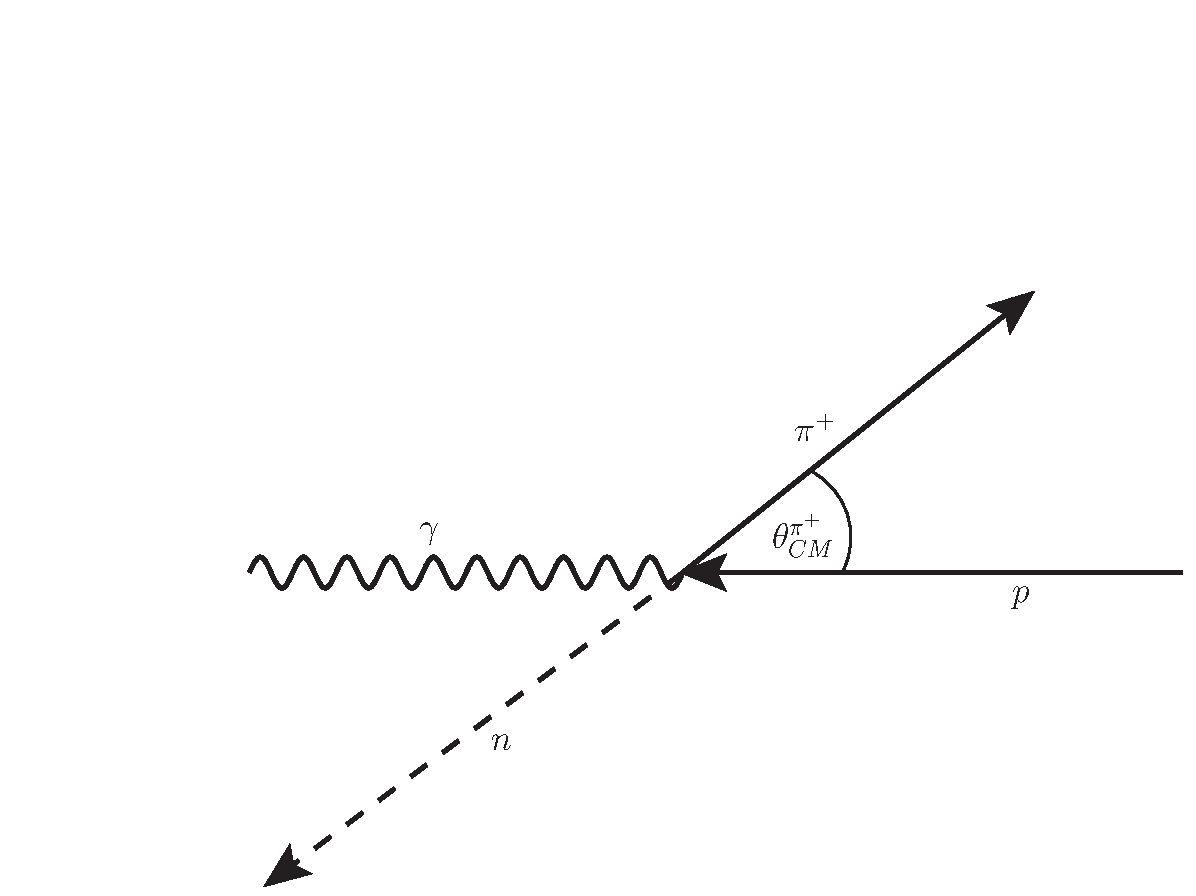
\includegraphics[width=0.6\textwidth]{figures/frost_reaction.pdf} \\
    \caption{The $\gamma p \rightarrow \pi^+ n $ reaction in the center of mass frame. }
    \label{fig:frost_diagram}
  \end{center}
\end{figure}
\begin{center}
\begin{tabular}{ |l||l|l||l|l||l|l||l|l||}
  \hline
  \multicolumn{9}{|c|}{g9a Run period: Linearly polarized } \\
  \hline
   \multicolumn{3}{|l||}{$E_{beam}$} & \multicolumn{6}{|c||}{2.780 GeV}   \\
  \hline
  \multicolumn{3}{|l||}{$Coh_{Edge}$} & \multicolumn{2}{|c||}{0.73 GeV} &  \multicolumn{2}{|c||}{0.93 GeV} &  \multicolumn{2}{|c||}{1.1 GeV}   \\
  \hline
 \multicolumn{3}{|l||}{} & $E_{CMS}^{min} $ &  $E_{CMS}^{max} $ & $E_{CMS}^{min} $ &  $E_{CMS}^{max} $ & $E_{CMS}^{min} $ &  $E_{CMS}^{max} $\\
\multicolumn{3}{|l||}{(GeV)} & 1.4 & 1.5 & 1.54 & 1.63 & 1.63 & 1.72  \\
 \hline
 \multicolumn{3}{|l||}{} & n  &  $\Delta E$ & n  &  $\Delta E$ & n  &  $\Delta E$ \\
\multicolumn{3}{|l||}{(MeV)} & 4 & 25 & 3 & 30 & 3 & 30  \\
    \hline
  \hline
$E_{beam}$&  \multicolumn{8}{|c||}{3.545 GeV} \\
  \hline
$Coh_{Edge}$&  \multicolumn{2}{|c||}{1.1 GeV} &  \multicolumn{2}{|c||}{1.3 GeV} &  \multicolumn{2}{|c||}{1.5 GeV} &  \multicolumn{2}{|c||}{1.7 GeV} \\
  \hline
& $E_{CMS}^{min} $ &  $E_{CMS}^{max} $& $E_{CMS}^{min} $ &  $E_{CMS}^{max} $ & $E_{CMS}^{min} $ &  $E_{CMS}^{max} $ & $E_{CMS}^{min} $ &  $E_{CMS}^{max} $ \\
(GeV) & 1.63 & 1.72 & 1.71 & 1.83 & 1.835 & 1.925 &  1.93 & 2.02 \\
 \hline
& n  &  $\Delta E$ & n  &  $\Delta E$ & n  &  $\Delta E$& n  &  $\Delta E$ \\
(MeV) & 3 & 30 & 4 & 30 & 3 & 30 &3 &30 \\
  \hline
  \hline
   \multicolumn{3}{|l||}{$E_{beam}$} &  \multicolumn{6}{|c||}{4.599 GeV} \\
  \hline
\multicolumn{3}{|l||}{$Coh_{Edge}$} &  \multicolumn{2}{|c||}{1.9 GeV} &  \multicolumn{2}{|c||}{2.1 GeV} &  \multicolumn{2}{|c||}{2.3 GeV}  \\
  \hline
 \multicolumn{3}{|l||}{} & $E_{CMS}^{min} $ &  $E_{CMS}^{max} $& $E_{CMS}^{min} $ &  $E_{CMS}^{max} $ & $E_{CMS}^{min} $ &  $E_{CMS}^{max} $ \\
\multicolumn{3}{|l||}{(GeV)} & 1.945 & 2.105 & 2.05 & 2.2 & 2.19 & 2.29 \\
 \hline
 \multicolumn{3}{|l||}{} & n  &  $\Delta E$ & n  &  $\Delta E$ & n  &  $\Delta E$ \\
\multicolumn{3}{|l||}{(MeV)} & 4 & 40 & 3 & 50 & 2 & 50  \\
  \hline
\end{tabular}
\end{center}

\subsection{Data Reduction}
The BOS files stored on the JLab tape silo contain all the data collected during JLab experiments so that they can be used for a wide range of analyses. Before the analysis of these data could begin a preliminary reduction of the g9a data set was carried out at JLab allowing the reduced files to be copied to the Edinburgh work disks and to also reduce the CPU time required for analysis. The CLAS analysis package, ROOTBEER \cite{rootbeer} was used for the preliminary data reduction process as well as for the subsequent analysis procedure described in this chapter. This is based on ROOT/C++ and interprets the bank structure of CLAS data. In this preliminary event selection two conditions determined the events which were retained:
\begin{enumerate}
\item  For each event, between one and three particles must be detected in conjunction with a hit in the tagger.
\item  Only three combinations of particles were allowed: one positive particle, one positive and one neutral particle, or one positive and two neutral particles. 
\end{enumerate}
The resulting files were then output as more compact ROOTDST (Data Summary Tape) files.

\subsection{The g9a Targets}
In g9a experiment there were three targets simultaneously in the beamline, as shown in Figure \ref{fig:target_draw}.
\begin{figure}[htb]
  \begin{center}
    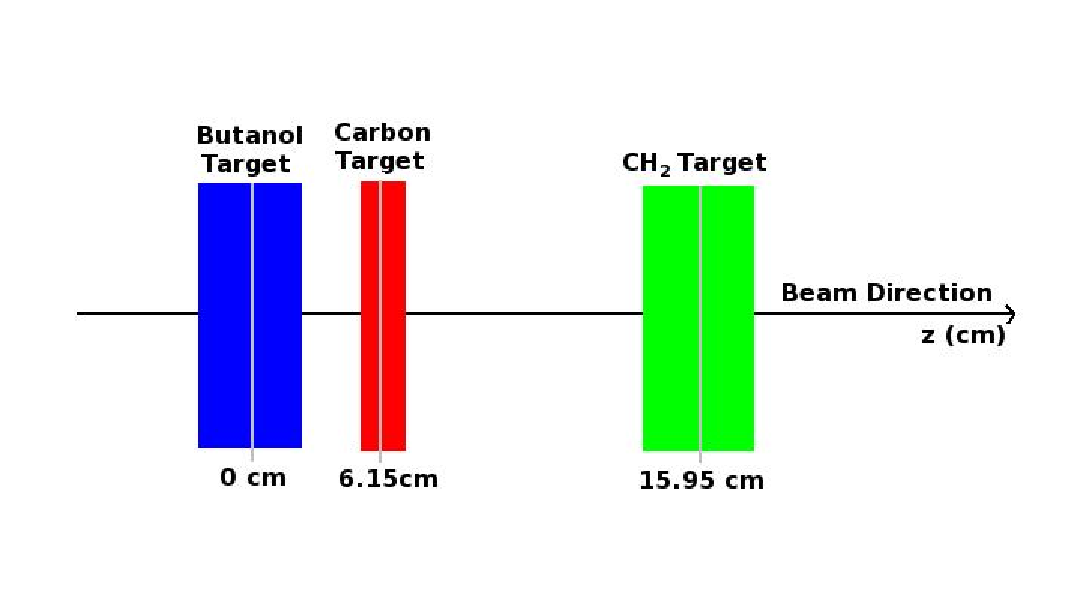
\includegraphics[width=0.6\textwidth]{figures/targets_drawing.png} \\
    \caption{Schematic diagram of the butanol, carbon and $CH_2$ targets in the beamline (not to scale) showing the position of their centres along the z axis. The butanol target was 2.67 mm thick, the carbon target was 1.49 mm thick and the $CH_2$ target was 3.45 mm thick. }
    \label{fig:target_draw}
    \end{center}
  \end{figure}
The butanol ($C_4 H_9OH$) target formed part of the FROST target system,  providing polarised protons. As butanol contains unpolarised carbon and oxygen atoms as well as polarised hydrogen, analysis of events originating within the carbon target allowed assessment of this unpolarised background contribution. The $CH_2$ target provides unpolarised protons, another useful cross-check for the analysis. Events from each of the three targets were selected by making a cut on the z-vertex position of each event to originate within one of the three targets. The z-vertex position is defined as the point of intersection of the beamline axis with the particle’s trajectory extrapolated back from the drift chambers. Figure \ref{fig:target_pos} shows the z-vertex position of all positive particle events along with the cuts made on the target positions as follows: -2.67 cm $\leq$ z $\leq$ 2.67 cm for the butanol target, 5.0 cm $\leq$ z $\leq$ 7.0 cm for the carbon target and 15.0 cm $\leq$ z $\leq$ 17.0 cm for the $CH_2$ target.
\begin{figure}[htb]
  \begin{center}
    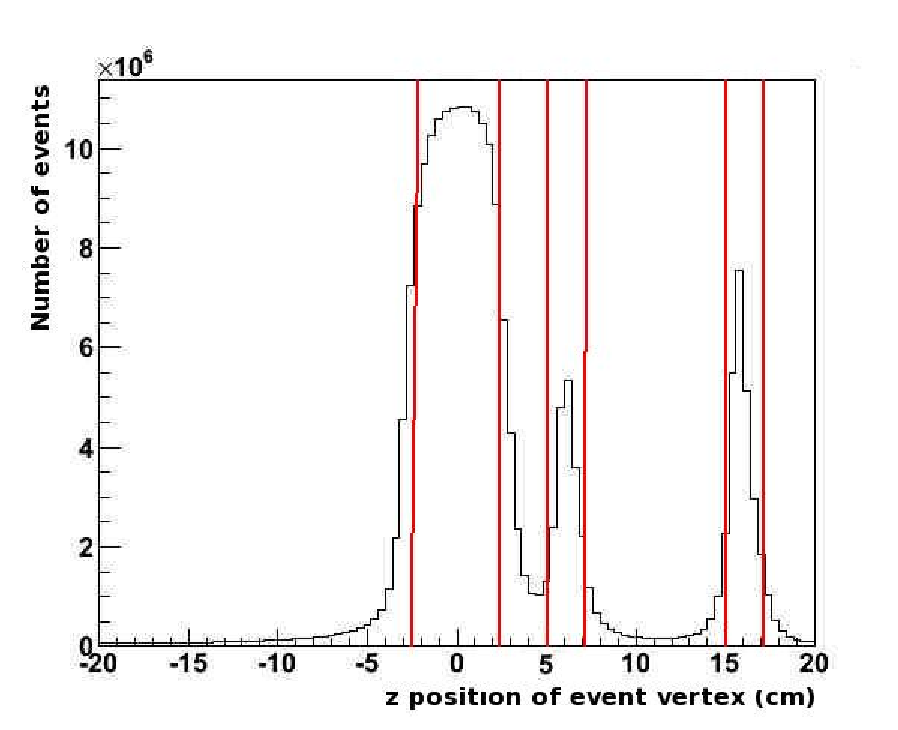
\includegraphics[width=0.6\textwidth]{figures/targets_pos.png} \\
    \caption{Z-vertex distribution of all positively charged particle events. The vertical red lines show the cuts made on the target positions as described in the text.}
    \label{fig:target_pos}
  \end{center}
\end{figure}



\subsection{Calculation of the Photon Beam Polarization}
To extract the G observable, as well as the other polarisation observables measured in this experiment, it was necessary to know the degree of linear beam polarisation as accurately as possible. The orientation of the polarisation plane must also be established with accuracy and can be determined from the goniometer settings. The calculation of the degree of linear beam polarisation involves comparing the shape of the coherent Bremsstrahlung spectrum to a spectrum obtained from theoretical Bremsstrahlung calculations. An enhancement plot can be used to separate the coherent contribution from the incoherent contribution to the spectra. The enhancement plots are fit with a theoretical spectrum produced by the Analytical Bremsstrahlung (ANB) Calculation \cite{Natter_2003}\cite{Sabin_2010}. The ANB calculation takes into account 17 experimental parameters characterising the geometry of the radiator, collimator and photon beam. Several of these parameters can be measured experimentally (such as photon beam energy and beam spot size) whereas others (such as electron beam divergence on the radiator) are varied until a good agreement is obtained between the enhancement plot and the ANB calculation. These parameters are then extracted from the fit and are used to calculate the degree of polarisation per event as a function of photon energy. This information is then summarised in lookup tables \cite{Anderson_table}.



\subsection{$\pi^+$ identification}
Different cuts were applied on the data in order to select events with a single $\pi^+$.
\begin{enumerate}
  \item number of photons in the same RF bucket = 1
  \item mass calculated from SC and TAG
  \item charge of track = +1
  \item The $\beta$ distribution was fitted for different momentum bins and a $\pm 3 \sigma$ cut was applied around the center of the distribution (see Fig. \ref{fig:beta_mom_pip} ) for particles with momentum $p_{\pi^+} < 1.2GeV$. For higher momentum, the statistic was poorer for clearly defining a $\pm 3 \sigma$ cut and no contamination was clearly seen in this range after all the cuts.
  \item  $\pm 3 \sigma$ cut around the $m^2$ of the pion
\end{enumerate}
\begin{figure}[htb]
  \begin{center}
    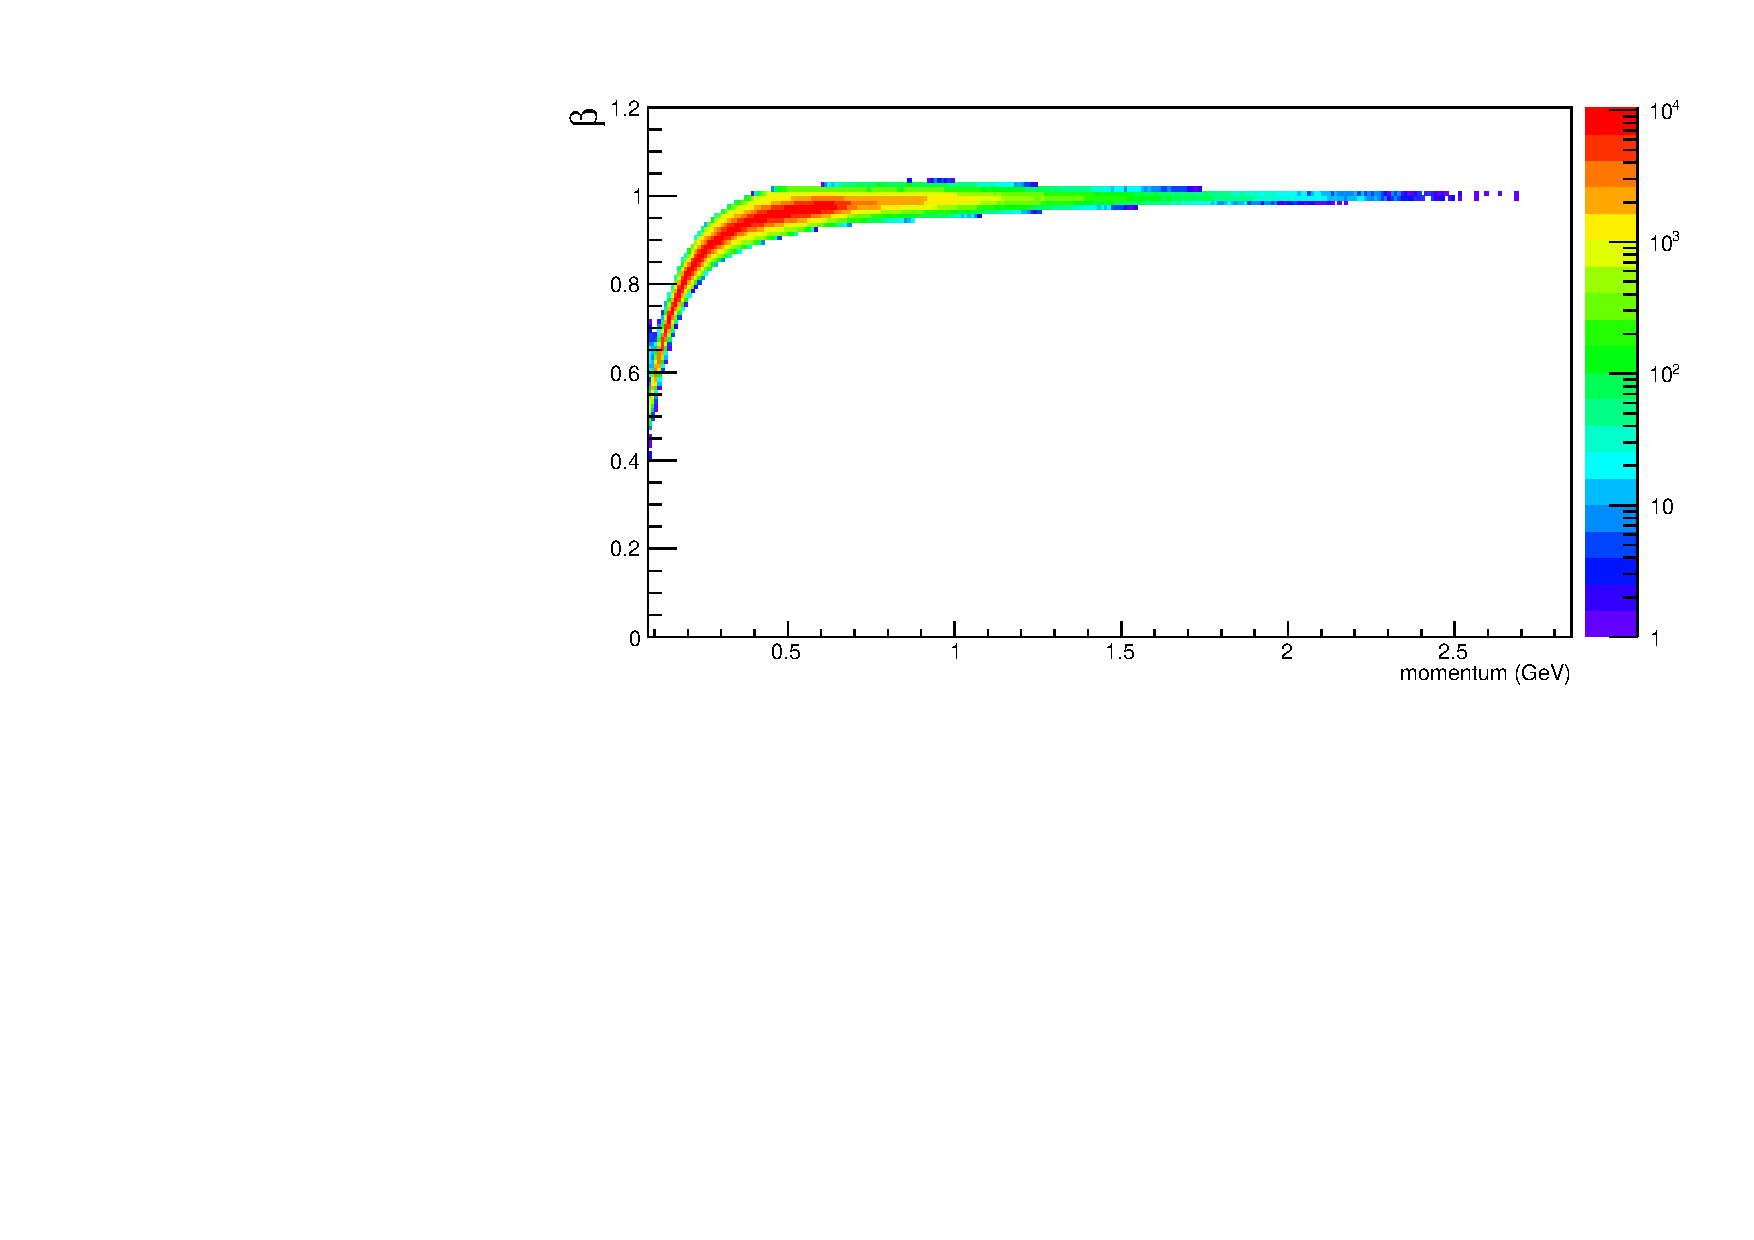
\includegraphics[width=0.6\textwidth]{figures/pid_beta_mom_pip.pdf} \\
    \caption{$\beta$ vs $momentum$ for selected $\pi^+$ tracks}
    \label{fig:beta_mom_pip}
  \end{center}
\end{figure}

\subsubsection{Pion-Photon Timing}
The time at which each event took place was now compared to the timing of the photon measured by the tagger. This allowed the reduction of background and accurate knowledge of the photon energy corresponding to each event as required for the missing mass calculation. The photons within the coherent peak were first selected using a simple cut on the photon energy range. The upper limit of this range was the coherent peak setting, the lower limit was the photon energy at which the beam polarisation dropped to 20\%. The arrival time of these photons at the event vertex, $t_\gamma$ , was then calculated using the tagger time, $t_{TAG}$, and the distance the photon travels from the radiator to the event vertex along the axis of the beamline, $z$ :
$$
t_\gamma = t_{TAG} + \frac{z}{c}
$$
The $\pi^+$ time, $t_\pi$, a the event vertex was then calculated as:
$$
t_\pi = t_{SC} - \frac{d}{c \beta_\pi}
$$
\begin{figure}[htb]
  \begin{center}
    \begin{tabular}{lr}
      \begin{minipage}{0.5\textwidth}
        \begin{flushleft}
          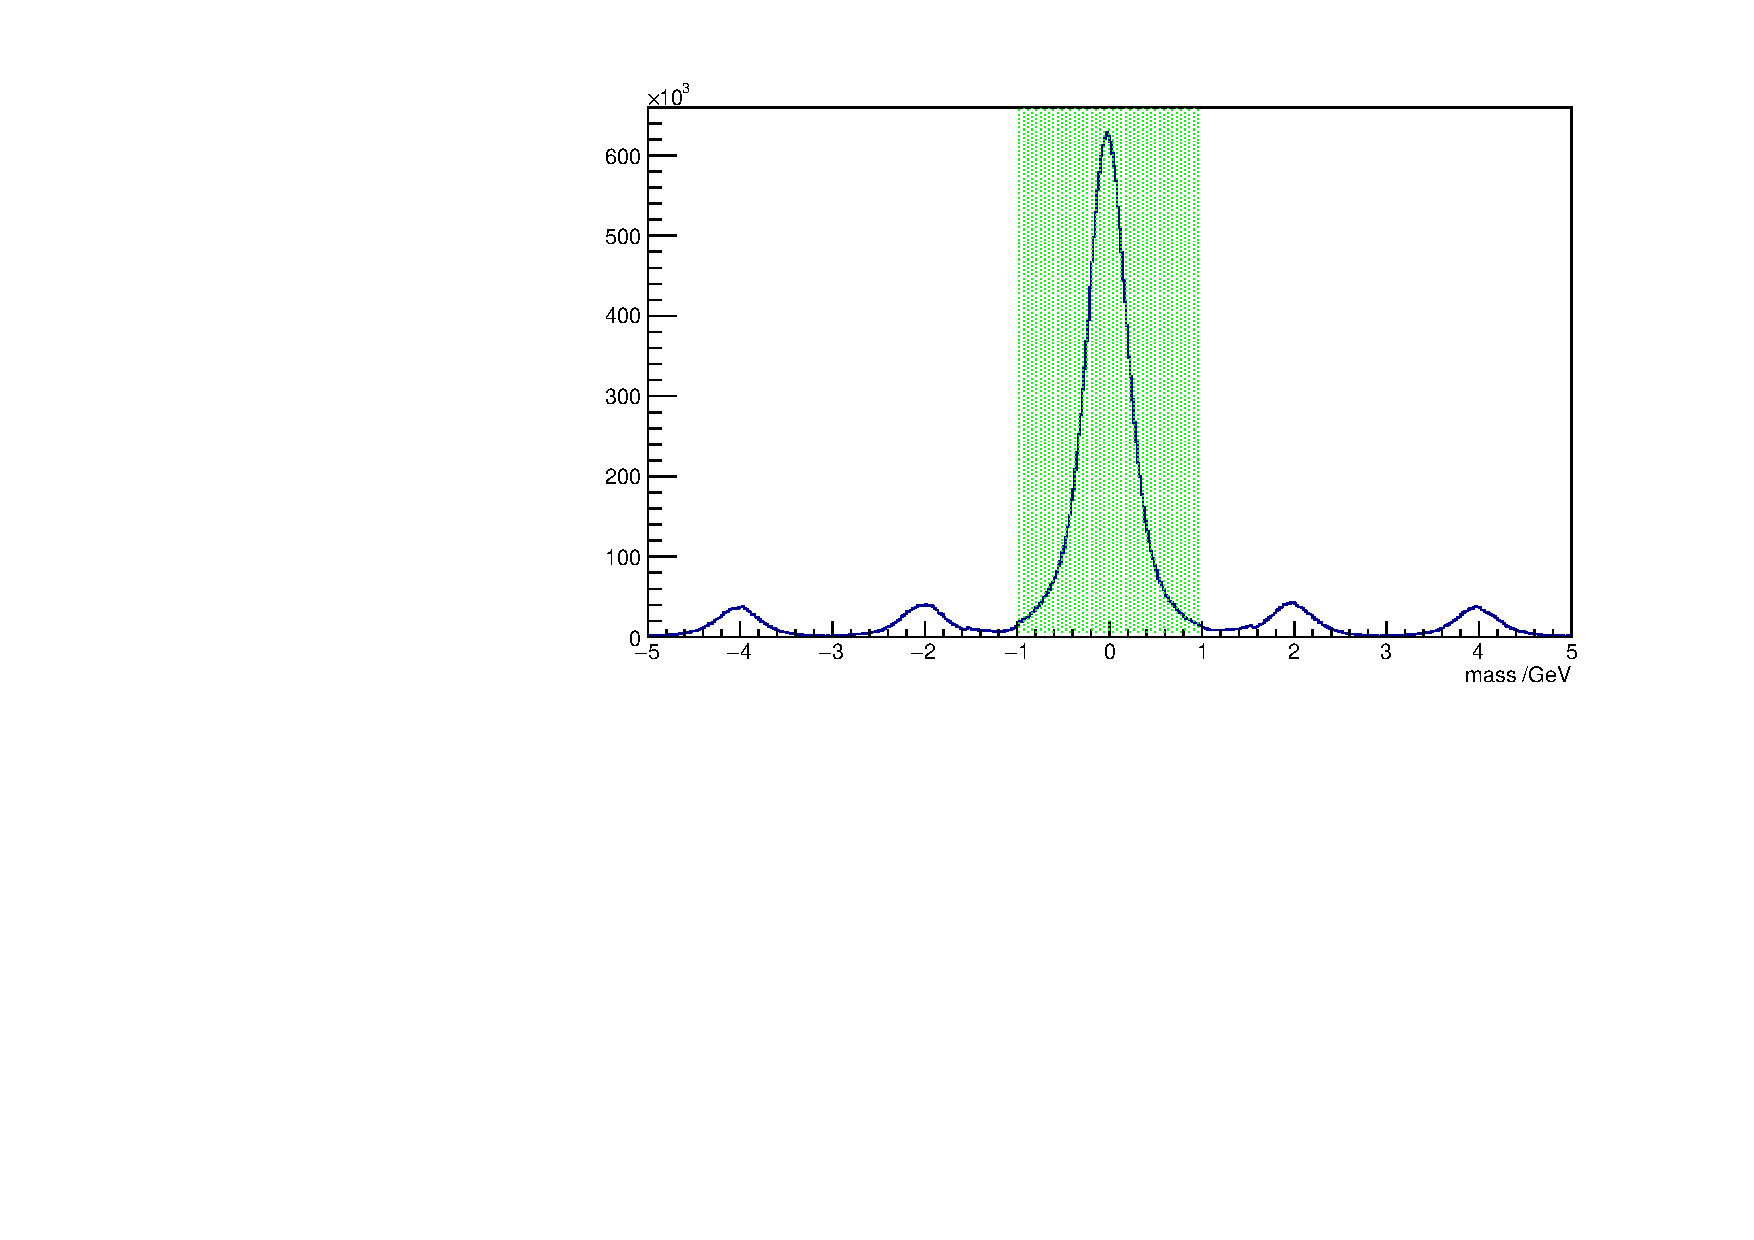
\includegraphics[width=0.95\textwidth]{figures/best_pion_photon_timing.pdf} \\
          \caption{Best Pion-photon timing}
          \label{fig:pion-photontiming}
        \end{flushleft}
        \end{minipage} &
        \begin{minipage}{0.5\textwidth}
        \begin{flushright}
          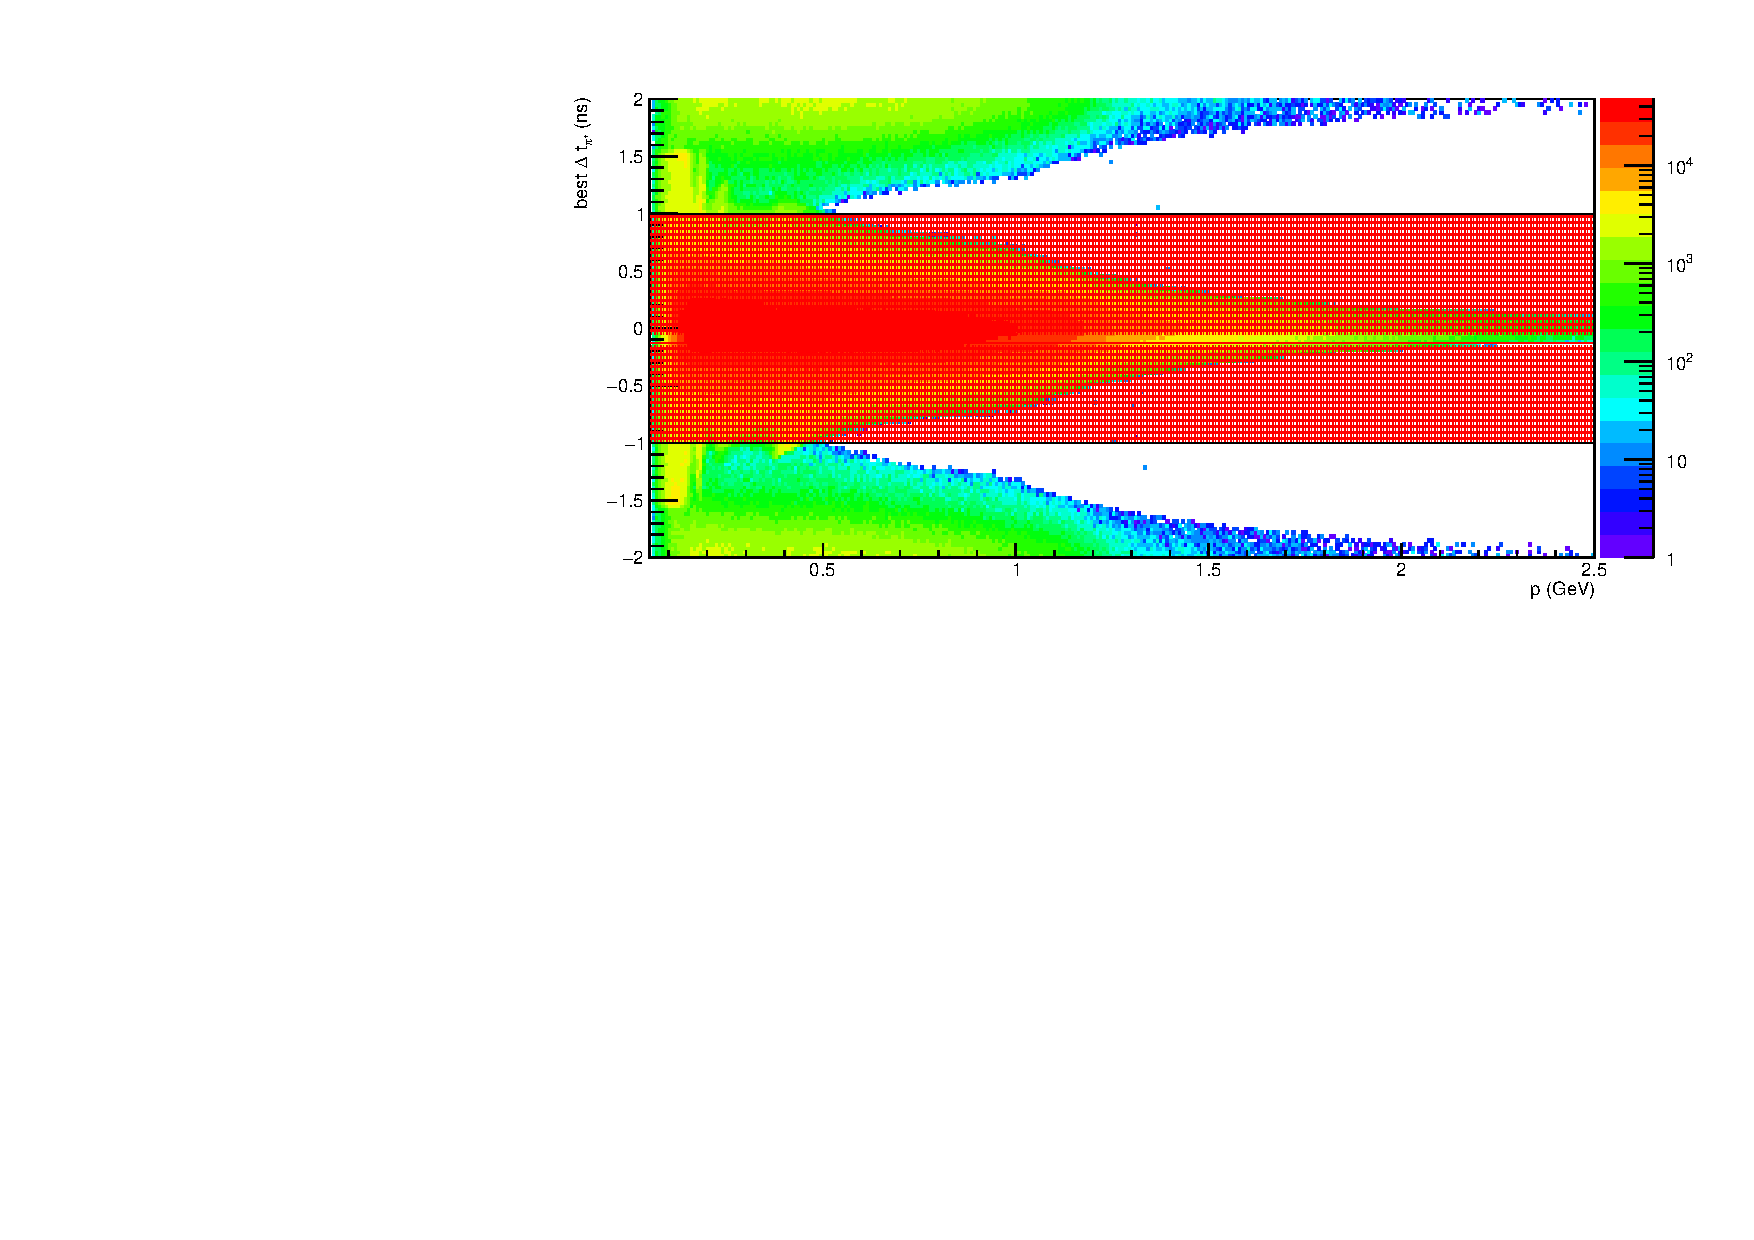
\includegraphics[width=0.95\textwidth]{figures/best_pion_photon_timing_vs_p.pdf} \\
          \caption{Best Pion-photon timing vs $\pi^+$ momentum}
          \label{fig:pion-photontiming_vsp}
        \end{flushright}
        \end{minipage}
    \end{tabular}
  \end{center}
\end{figure}
where $t_{SC}$ is the time recorded for the event by the Start Counter, $d$ is the distance between the event vertex and the hit position in the Start Counter  and $\beta_\pi = \sqrt{\frac{p^2}{m^2 + p^2}} $.  The event photon was defined as the photon whose vertex time is closest to the $\pi^+$ vertex time. Fig. \ref{fig:pion-photontiming} shows the time difference between these event photons and the $\pi^+$ vertex time, $\Delta t$ , with the majority of events having a time difference centred on zero. The smaller peaks to either side of the main peak correspond to photons from other beam buckets which were recorded during the time-window of the trigger for each event. These photons arising from neighbouring beam buckets were removed by setting the condition that 
\begin{enumerate}
\item $\Delta t$ must be within $1 ns$. 
\item One single photon in this timing region per event
\end{enumerate}


\subsubsection{Energy Loss Corrections}

The four-momentum of the $\pi^+$ is determined, in part, by the three-momentum obtained from the $\pi^+$ tracks in the drift chambers. This measured momentum does not take into account the energy losses of the particles as they pass through the target cell walls, mixing chamber and holding coil as well as the start counter before entering the drift chambers. As a result, the momentum of the $\pi^+$ can be up to $\sim 0.02 GeV/c$ higher than that measured, as shown in Figure 8.8.
The data were corrected for this loss in momentum using the ELOSS package [147] which was updated for the g9a. This is the standard energy-loss correction software for CLAS experiments and can be applied to any charged particle with a mass greater than that of an electron. The target geometry, event vertex position and particle four-momentum is input into ELOSS which then tracks back the flight path of the particle from the point at which it entered the Region 1 Drift Chambers to the event vertex. The path length of the particle in each of the materials it traverses is obtained allowing the energy lost in each material and hence the momentum lost by the particle to be calculated. The mass and energy of the $\pi^+$ were now recalculated using the energy-loss corrected values of momentum, the PDG value of $\pi^+$ mass and the measured value of beta (Equations 8.3 and 8.4). A new energy-loss corrected four-vector was therefore created for the $\pi^+$ which was then applied in the missing mass calculation described in the next section.
\begin{figure}[htb]
  \begin{center}
    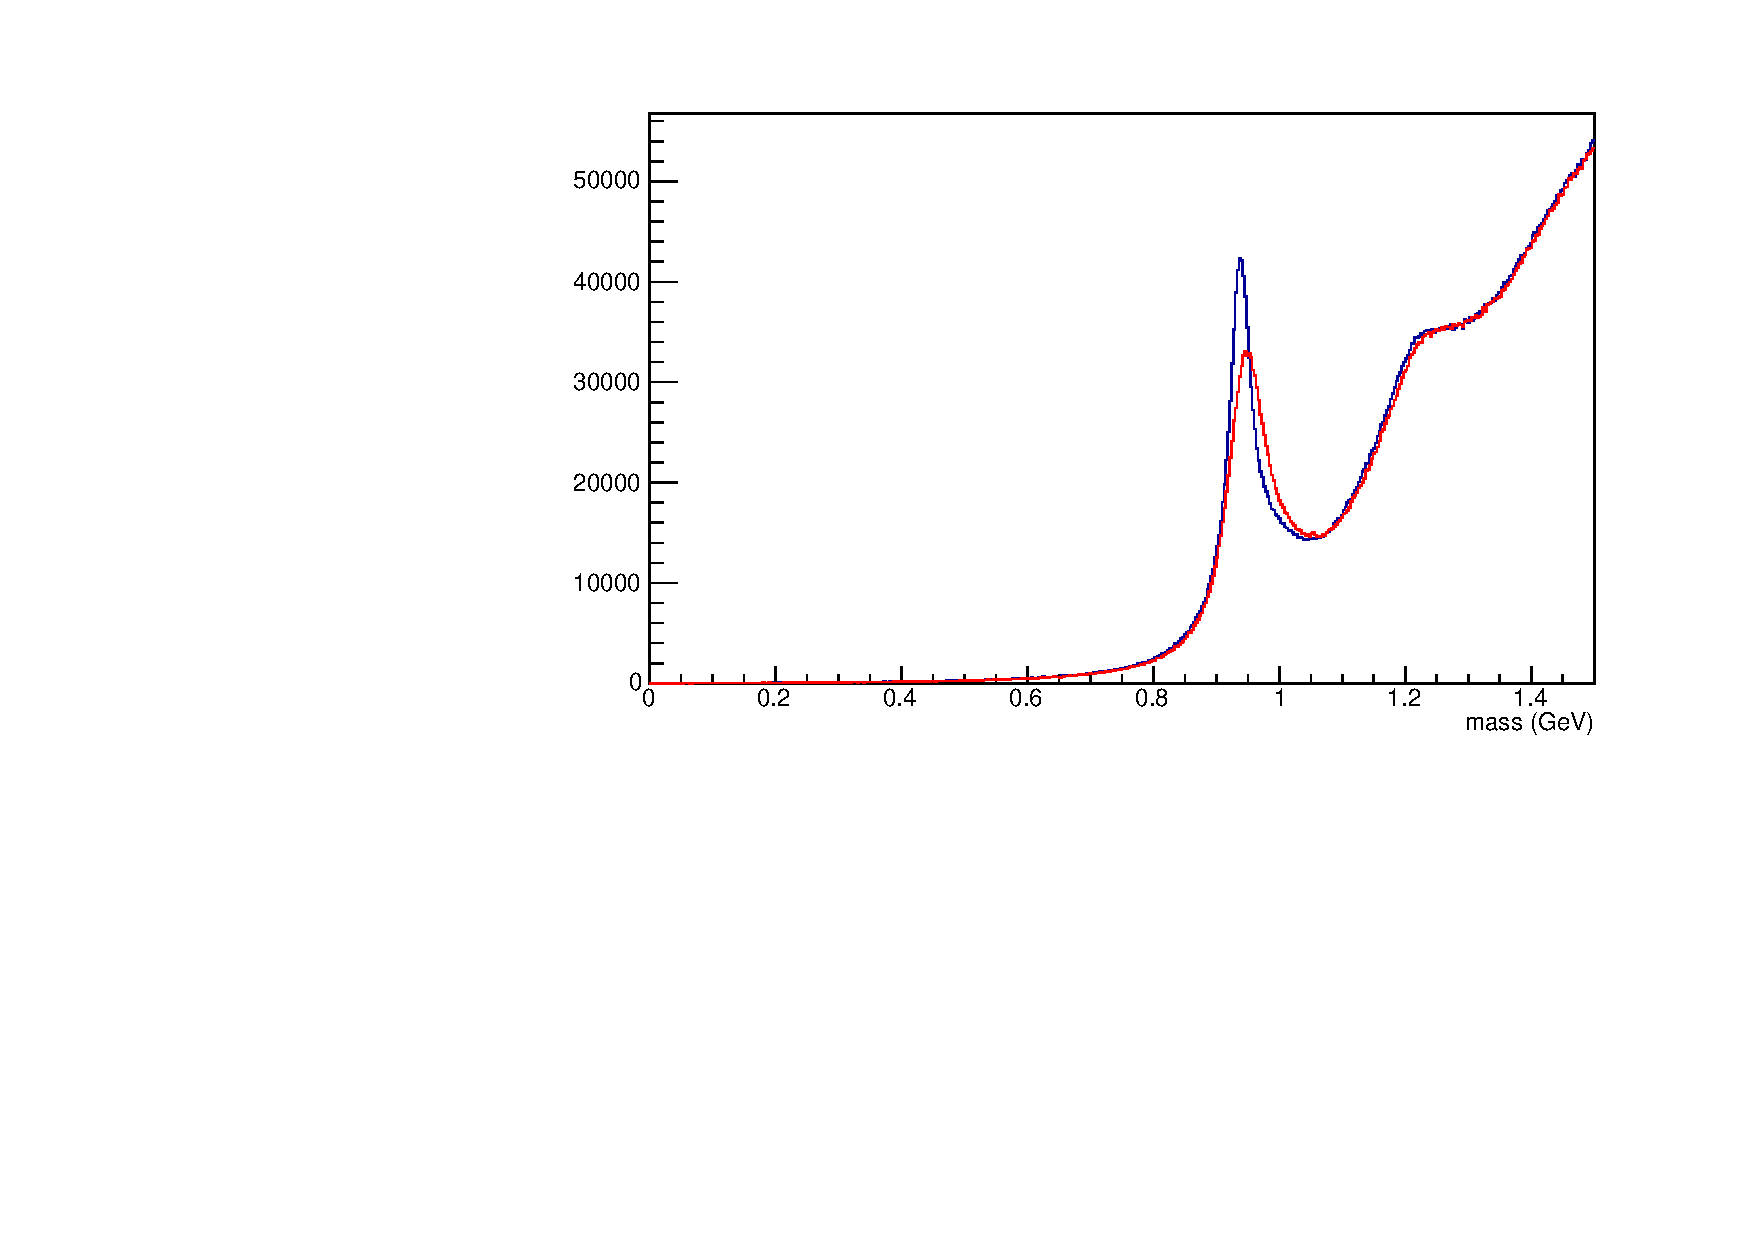
\includegraphics[width=0.6\textwidth]{figures/eloss_comp.pdf} \\
    \caption{Reconstructed Mass of the neutron before (red) and after eloss (blue)}
    \label{fig:eloss_comp}
  \end{center}
\end{figure}



\section{Extraction of the G Double-Polarization Observable}
The Cross section for this reaction, considering the target linear Polarization along the photon beam direction $P_z$, and the Polarization of the photon beam ($P_{\parallel}$ (Electric field parallel to the floor) and $P_{\perp}$ (Electric field perpendicular to the floor)), can be written as:
\begin{equation}
\frac{d\sigma}{d\Omega} = \left(\frac{d\sigma}{d\Omega}\right)_{UNPOL}  \left( 1 + P_{\gamma}\Sigma cos(2\phi) + P_{\gamma} P_z G sin(2\phi) \right)
\end{equation}

During the g9a run period all the possible combinations of different polarizations where measured, reaching the full configuration

\begin{eqnarray}
\left(\frac{d\sigma}{d\Omega}\right)_{\parallel +} = \left(\frac{d\sigma}{d\Omega}\right)_{UNPOL}  \left( 1 + P_{\gamma \parallel}\Sigma cos(2\phi) + P_{\gamma \parallel} P_{+z} G sin(2\phi) \right) \\
\left(\frac{d\sigma}{d\Omega}\right)_{\parallel -} = \left(\frac{d\sigma}{d\Omega}\right)_{UNPOL}  \left( 1 + P_{\gamma \parallel}\Sigma cos(2\phi) - P_{\gamma \parallel} P_{-z} G sin(2\phi) \right) \\
\left(\frac{d\sigma}{d\Omega}\right)_{\perp +} = \left(\frac{d\sigma}{d\Omega}\right)_{UNPOL}  \left( 1 - P_{\gamma \perp}\Sigma cos(2\phi) - P_{\gamma \perp} P_{+z} G sin(2\phi) \right) \\
\left(\frac{d\sigma}{d\Omega}\right)_{\perp -} = \left(\frac{d\sigma}{d\Omega}\right)_{UNPOL}  \left( 1 - P_{\gamma \perp}\Sigma cos(2\phi) + P_{\gamma \perp} P_{-z} G sin(2\phi) \right)
\end{eqnarray}
An asymmetry between these configurations will permit to extract the desired parameter $G$. In order to normalize these measurement before calculating the asymmetry, the cross section was also calculated with the same configurations for the Polarized target, but with an amorphous crystal (Carbon), in order to create an unpolirized photon beam. This will also remove effects due to the acceptance of the detector. 

\subsection{Calculation of the flux on target, F}
During the experiment, every effort was made to collect the same amount of data for all four possible combinations of polarised beam-polarised target settings. In practice, however, the flux incident on the target for the PARA and PERP beam settings was not equal and the $\pi^+$ azimuthal distributions had to be scaled to each other before any further analysis.
\begin{figure}[htb]
  \begin{center}
    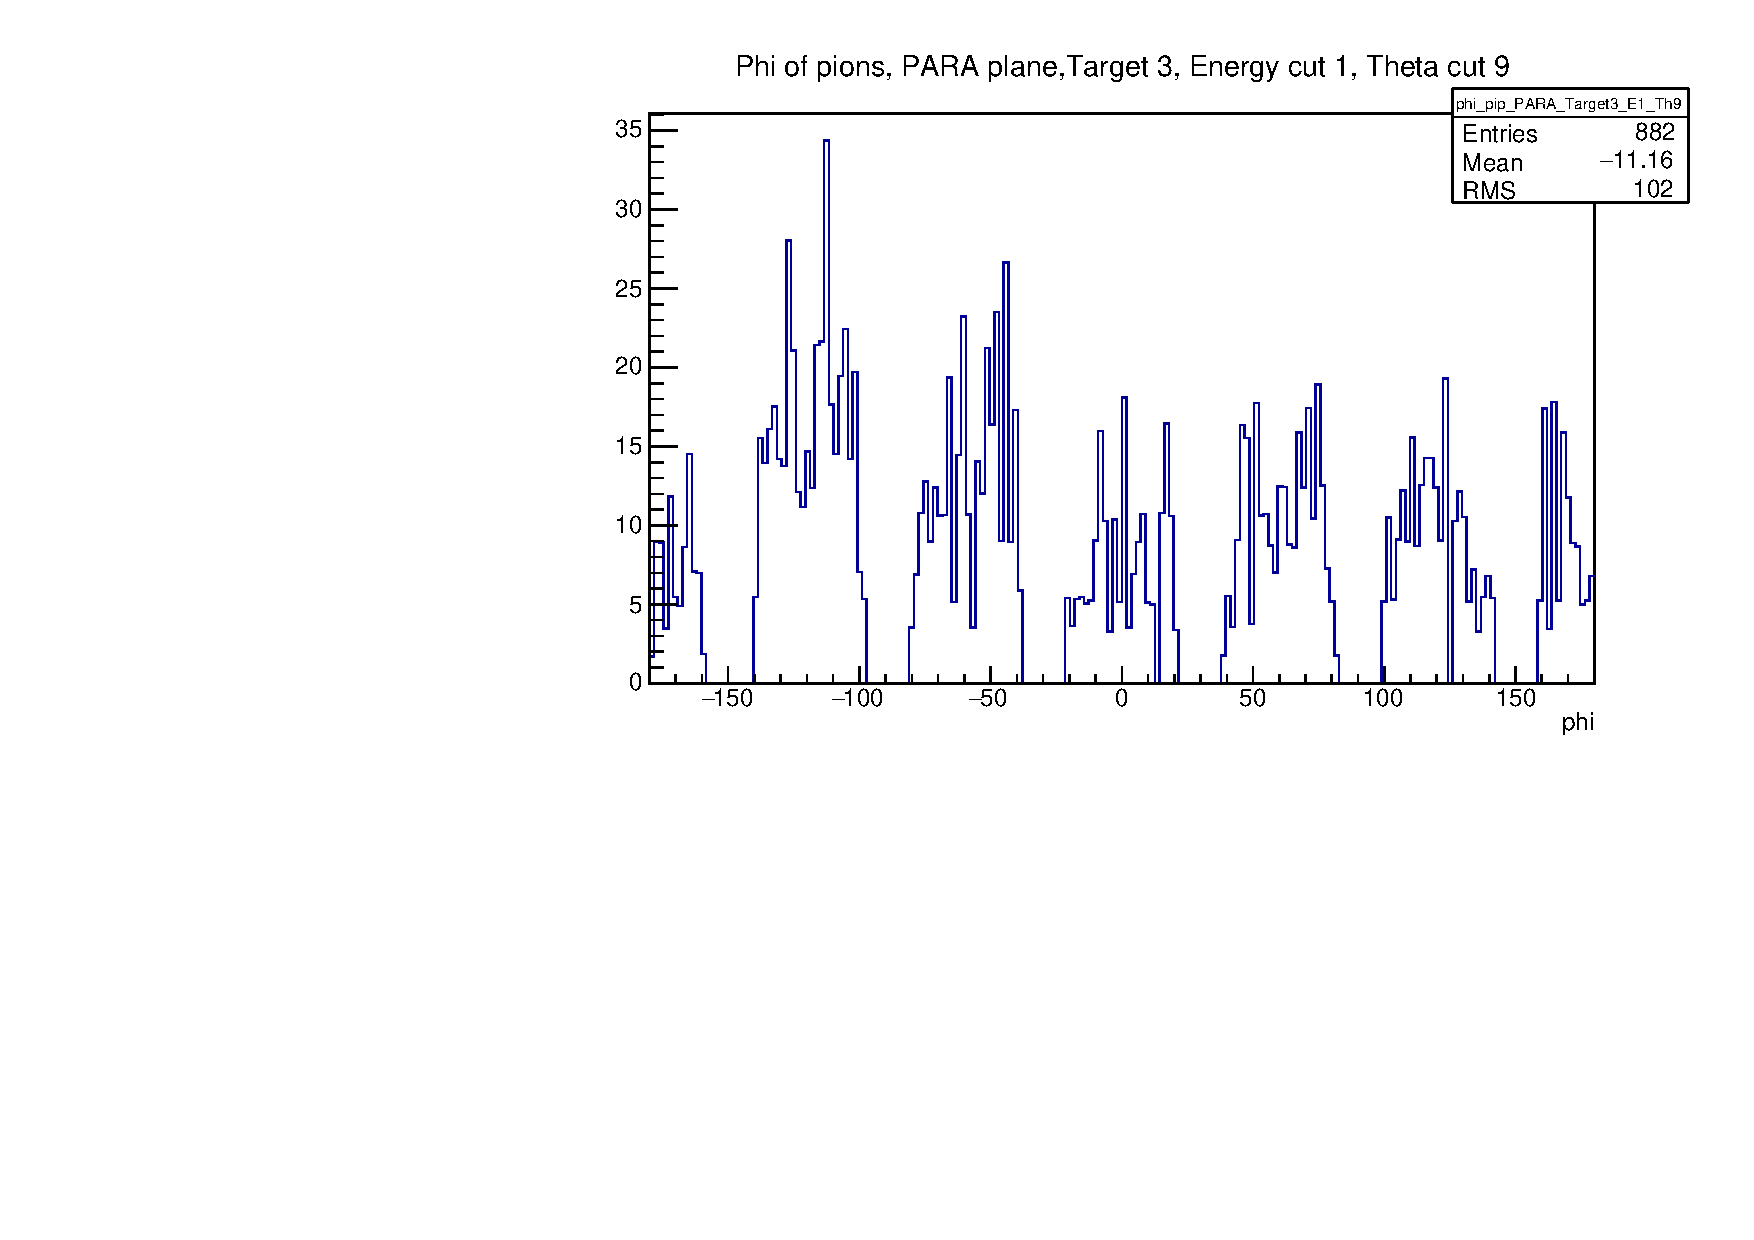
\includegraphics[width=0.6\textwidth]{figures/phi_PARA.pdf} \\
    \caption{$\phi$ distribution for PARA events for a single energy bin and $cos(\theta_{CM})$ bin. }
    \label{fig:frost_PARA_ex}
  \end{center}
\end{figure}



The PARA and PERP $\pi^+$ distributions for a particular target setting were first divided through by the AMO data to remove acceptance effects.
Considering now as:
\begin{enumerate}
  \item $F$ is the flux on target for each beam setting, which is dependent on both energy and linear beam polarisation. 
  \item $\phi_0$ is the “phi-offset” which accounts for any small mis-alignment of the diamond resulting in the beam polarisations not being exactly parallel or exactly perpendicular to the floor.
\end{enumerate}

\begin{eqnarray}
N_{\parallel +} = \frac{F_{\parallel}}{F_{AMO}} \left( 1 + P_{\gamma \parallel}\Sigma cos(2(\phi-\phi_0)) + P_{\gamma \parallel} P_{+z} G sin(2(\phi-\phi_0)) \right) \\
N_{\parallel -} = \frac{F_{\parallel}}{F_{AMO}} \left( 1 + P_{\gamma \parallel}\Sigma cos(2(\phi-\phi_0)) - P_{\gamma \parallel} P_{-z} G sin(2(\phi-\phi_0)) \right) \\
N_{\perp +} = \frac{F_{\perp}}{F_{AMO}} \left( 1 - P_{\gamma \perp}\Sigma cos(2(\phi-\phi_0)) - P_{\gamma \perp} P_{+z} G sin(2(\phi-\phi_0)) \right) \\
N_{\perp -} = \frac{F_{\perp}}{F_{AMO}} \left( 1 - P_{\gamma \perp}\Sigma cos(2(\phi-\phi_0)) + P_{\gamma \perp} P_{-z} G sin(2(\phi-\phi_0)) \right) \\
\end{eqnarray}
\begin{figure}[htb]
  \begin{center}
    \subfloat[][Asymmetry for $1.71GeV \leq E_{CM} < 1.74GeV$ and \\$0.4 \leq cos(\theta_{CM}) < 0.6$  ] {
      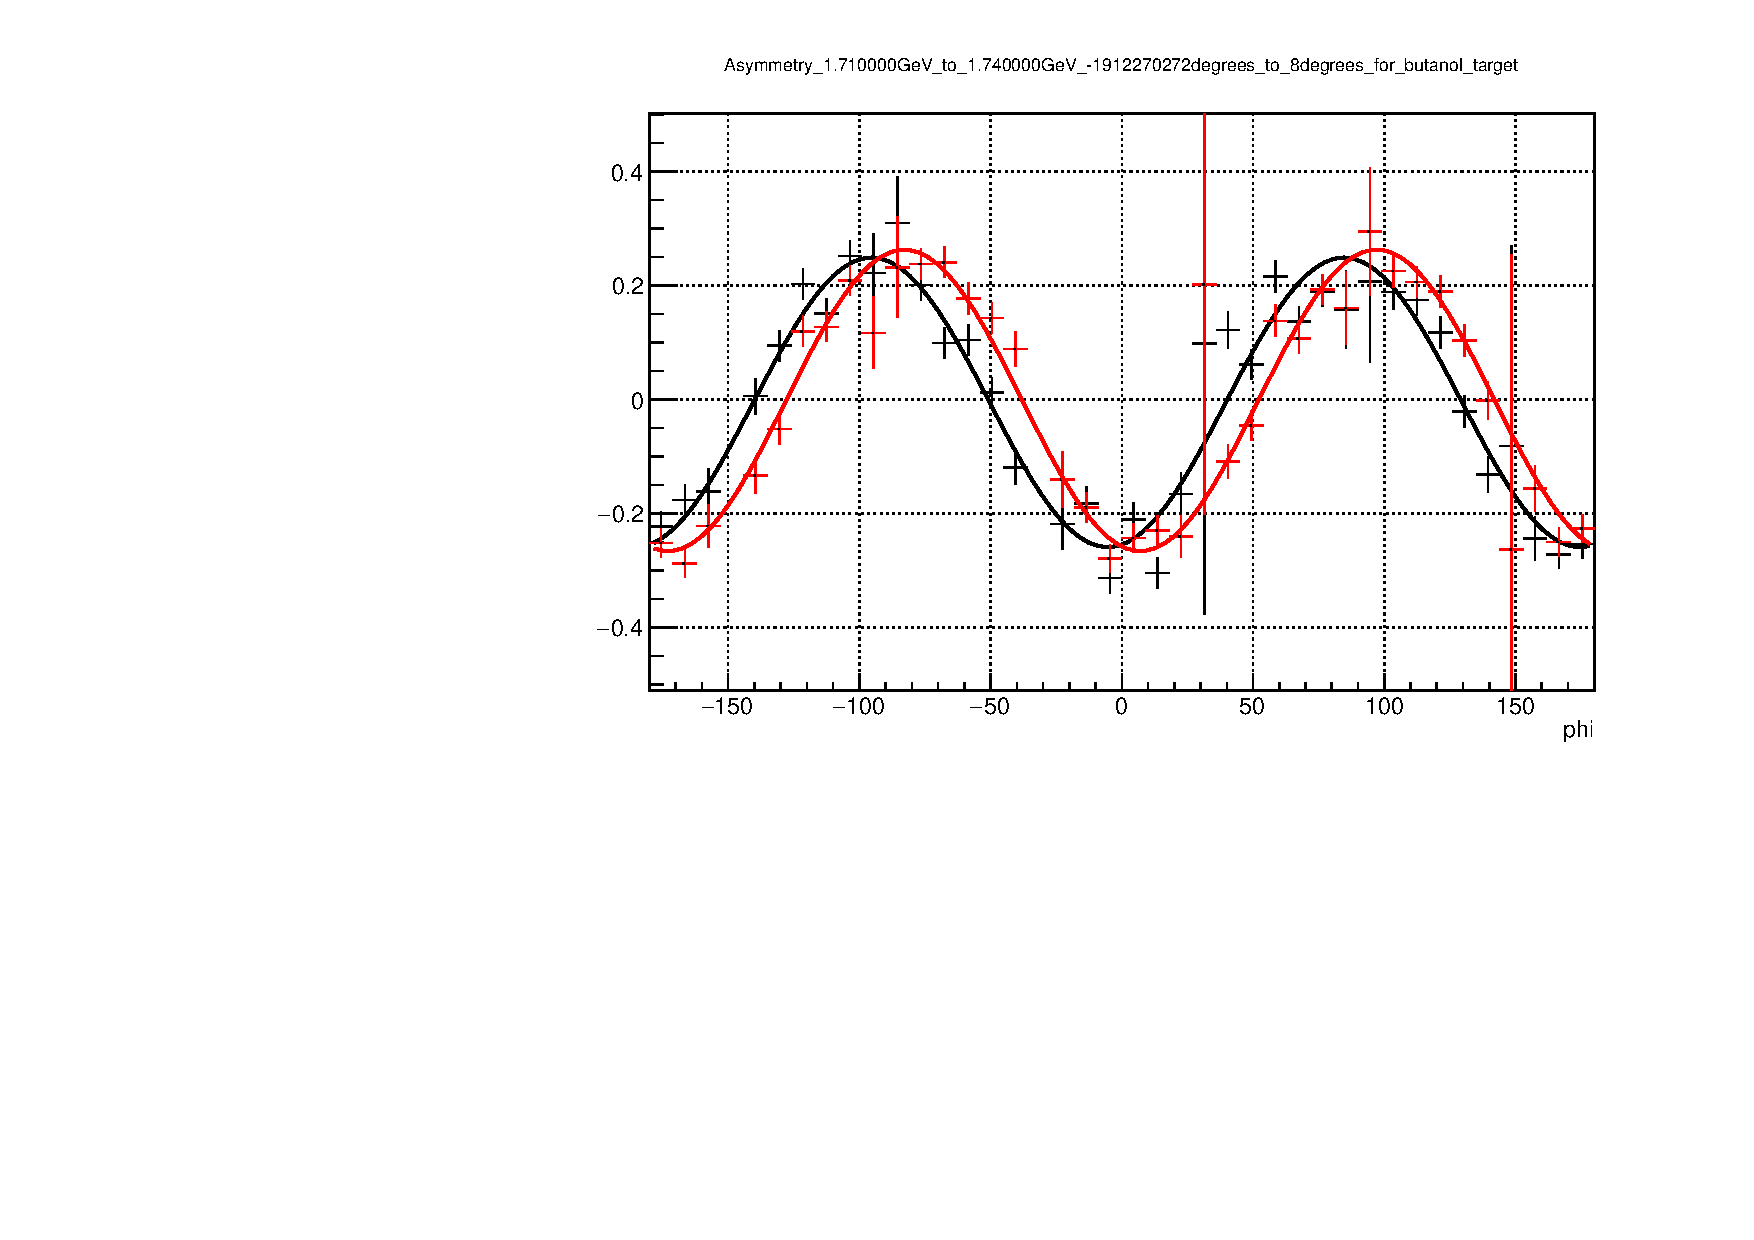
\includegraphics[width=0.5\textwidth]{figures/G_tgpol_effect.pdf} 
      \label{fig:GTgpol_theta1}
    }
    \subfloat[][Asymmetry  $1.54GeV \leq E_{CM} < 1.57GeV$ and \\$-0.6 \leq cos(\theta_{CM}) < -0.4$] {
      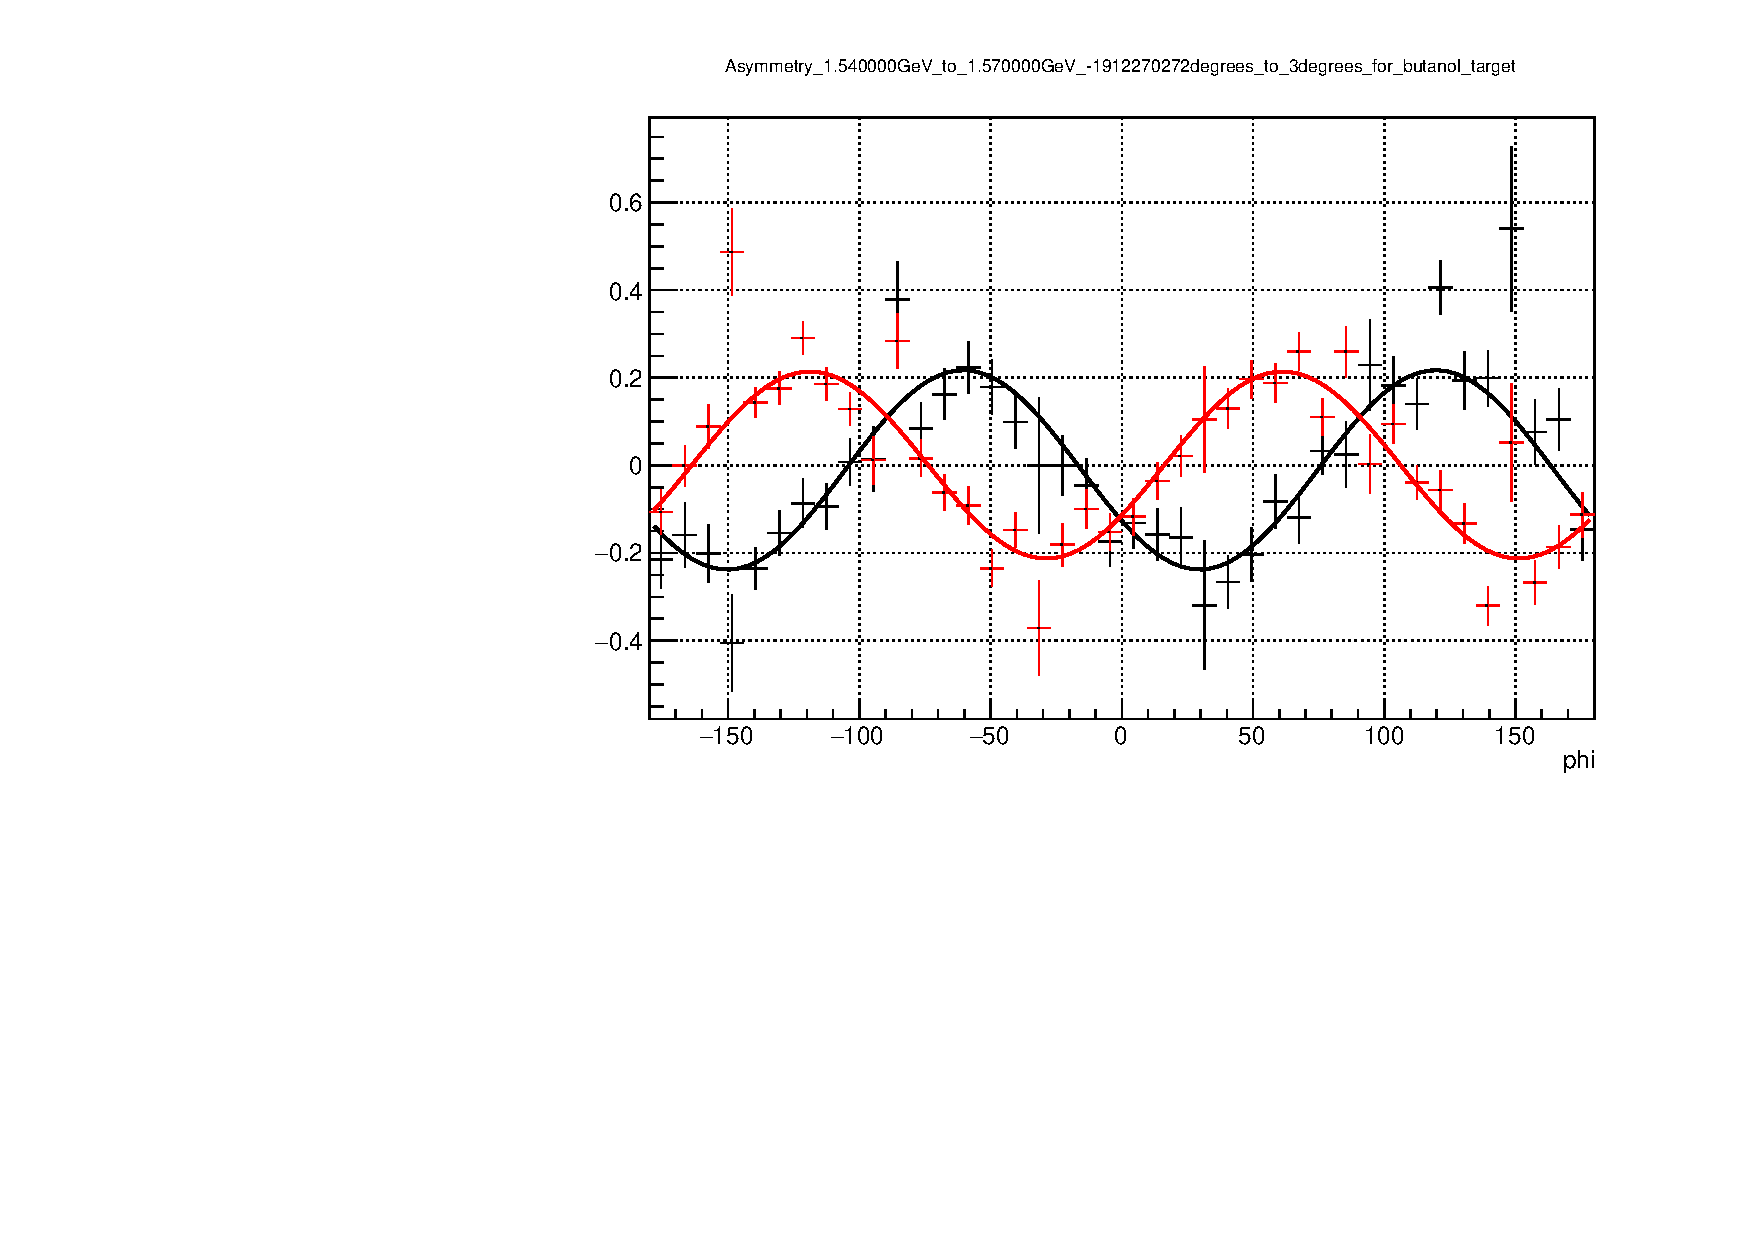
\includegraphics[width=0.5\textwidth]{figures/G_tgpol_effect2.pdf}
    \label{fig:GTgpol_theta2}
    } 
    \caption{The Asymmetry histogram with the fit is plotted for the two different target polarization. One can see the simmetry of the shift from the nominal position in the center ($\phi = 0$).  One can see that, still after the weighting with the Amorphous flux, there is still some effect due to lack of acceptance in the part separating the 6 sectors of CLAS}
  \end{center}
\end{figure}

These distributions where fitted with a function with 4 parameters ($ a,b,c,d $) :
\begin{equation} \label{eqn:fit_flux}
f(\phi) = a \{ 1 + b\, cos[2 (\phi - c) ]  + d\, sin[2(\phi - c)] \} 
\end{equation}
In this fit, $a$ will be directly related to the value that will be use to normalize the PERP and PARA fluxes and $c$ will be a check of the possible $\phi_0$ offset for possible diamond misalignement.
This method of dividing by the amorphous data rather than forming an asymmetry was necessary to allow the PARA and PERP flux to be extracted separately. In order to minimise the statistical error, this calculation was performed for each energy bin. The fit was optimised by calculating first $\phi_0$ and then fixing this value in the fit. 
Using the results of the fits for the PARA ($\parallel$) and PERP ($\perp$) configurations, the ratio between the two different measurements can be determined (using eqn. \ref{eqn:fit_flux}) as:
\begin{equation}
\frac{F_{\perp}}{F_{\parallel}} = \frac{a_{\perp}}{a_{\parallel}}
\end{equation}

\subsection{Calculation of Dilution Factor}
The dilution factor was calculated for each energy and for each $cos(\theta_{CM}$ bin using data obtained from the carbon target to model the unpolarised nucleon background in the butanol target.
As the four vectors of the incident photon, target proton and outgoing pion were known, the neutron four-vector was reconstructed using the missing mass technique:
$$
\gamma \, + \,  p \, \rightarrow \, \pi^+ \, + \, X
$$
\begin{figure}[htb]
  \begin{center}
    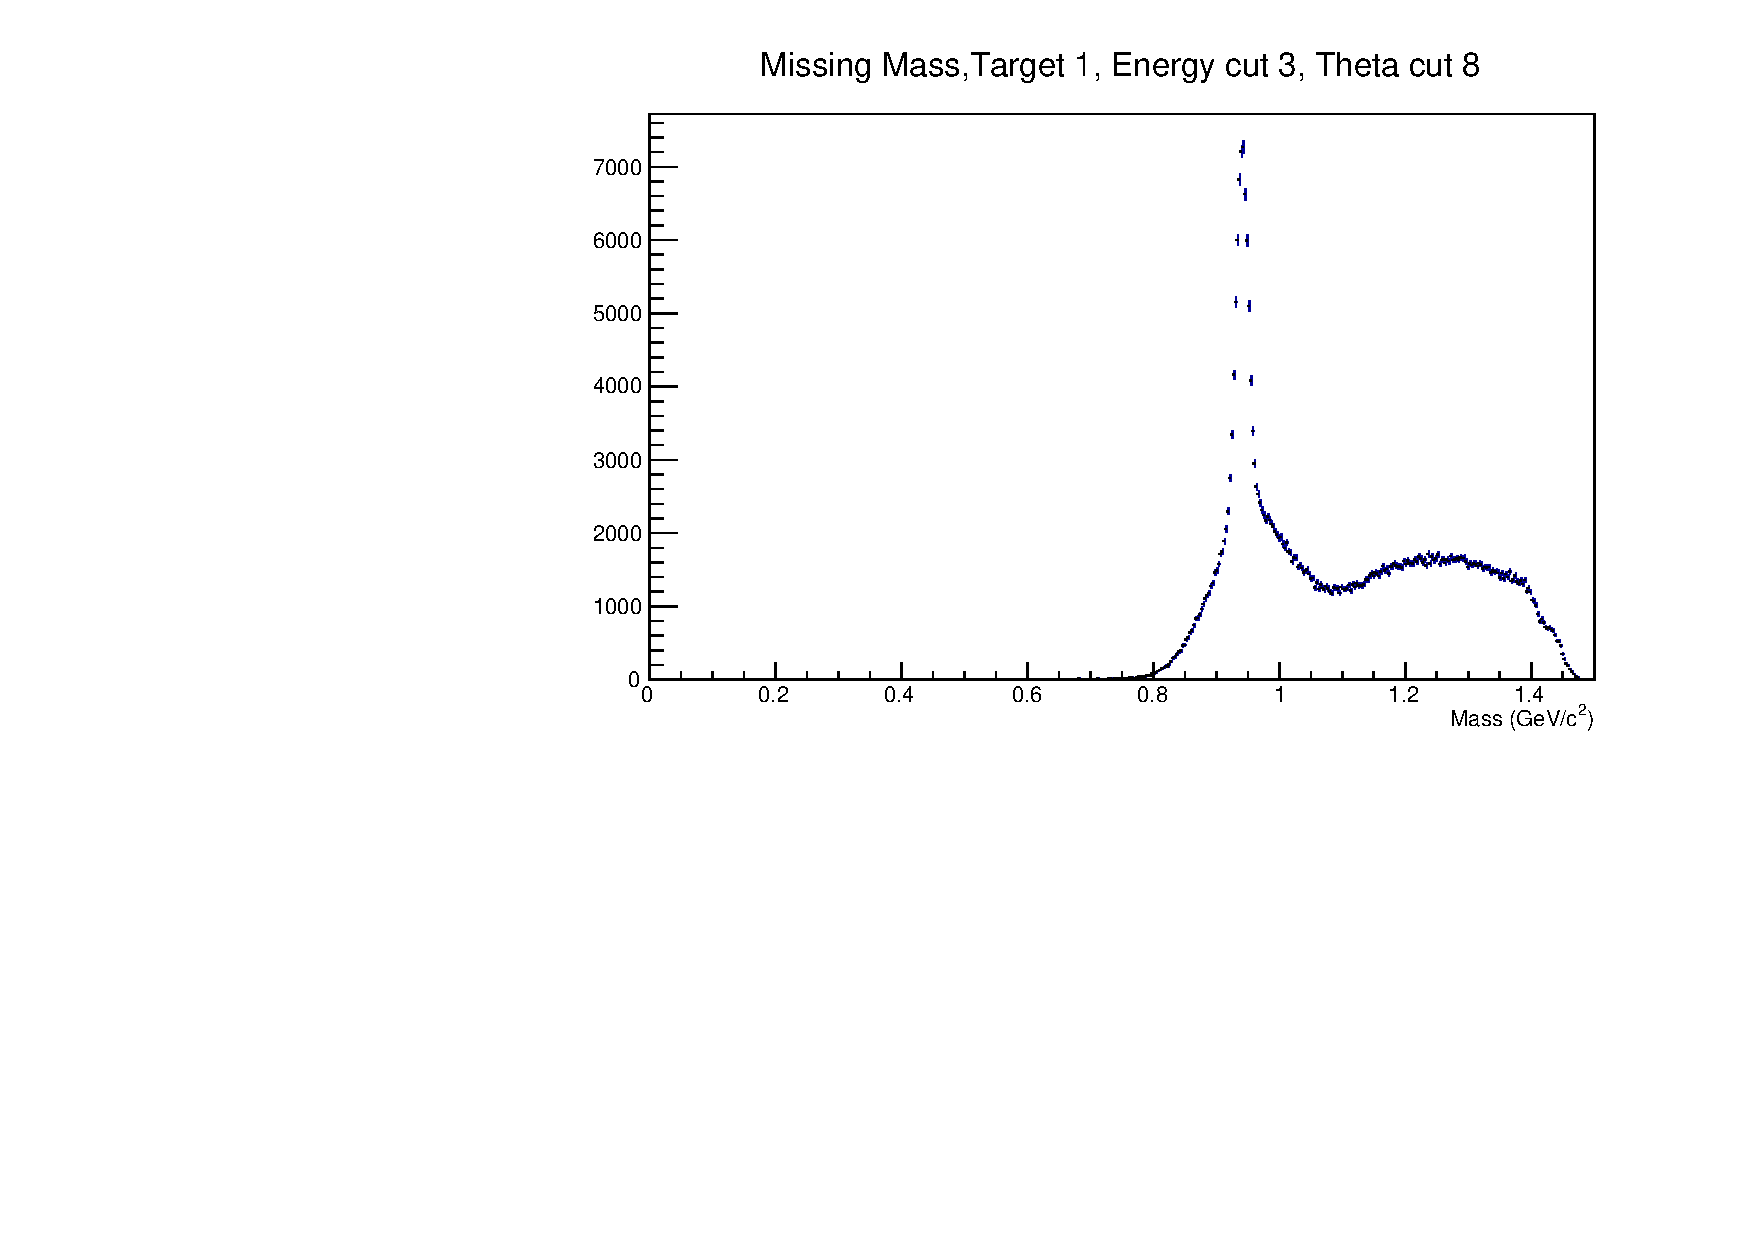
\includegraphics[width=0.6\textwidth]{figures/neutron_missingmass.pdf} \\
    \caption{Mass distribution obtained from the reconstructed neutron four-vector, showing a sharp peak corresponding to the reconstructed neutron and
a broad peak to the right of this corresponding mainly to two-pion production channels. }
    \label{fig:frost_neutronmissing_ex}
  \end{center}
\end{figure}
assuming momentum is conserved in this reaction. Here X can represent the neutron, other neutral particles, or combinations of positively and negatively charged particles such as $\pi^+ , \pi^-$. Figure --- shows the missing mass distribution obtained from the reconstructed neutral four-vector, showing a sharp peak corresponding to the missing neutron mass and a broad peak to the right of this corresponding to other possible channels such as multi-pion production. This plot also shows background contributions due to photon interactions with the carbon and oxygen atoms in the butanol target.
A mass cut was performed to select the neutron and hence the $\pi + n$ events of interest. The width of the neutron-mass squared cut was determined by making a rough subtraction of the carbon and oxygen background using the missing mass distribution obtained from the carbon target data. The missing-mass squared distribution obtained from the carbon target was first scaled to the butanol missing-mass distribution. To obtain the scale factor, the butanol missing mass spectrum was divided by the carbon missing mass spectrum and fit with a Gaussian function in the region of the neutron peak and a zeroth order polynomial in the region to the left of this peak as shown in Figure ---.
As the carbon and butanol targets were very close together in the beamline and could not be fully resolved in the z-vertex distribution spectrum, some events within the carbon z-vertex cuts will have originated from polarised protons within the butanol target.
The carbon missing-mass distribution shown in Figure --- was therefore fit with a combination of two Gaussian functions and a third order polynomial in order to model its shape as shown in Figure ---. One Gaussian function modelled the hydrogen “contamination”, the position and width being taken from the Gaussian fit to the carbon-subtracted butanol missing-mass distribution. The second Gaussian function represented the neutron peak due to the photon interaction with the carbon and oxygen nuclei. Neutron events originating from the photon interaction with a carbon or oxygen nucleus in butanol would be expected to form a peak similar in shape to the neutron peak corresponding to events from the hydrogen atom, but broadened due to the Fermi motion of the nucleons in the carbon or oxygen nucleus. The polynomial modelled the broad background coming from mostly multi-pion production and other non quasi-free processes.
Figure --- shows the butanol missing-mass distribution overlaid with a function representing only the quasi-free background in butanol, and so including only the Gaussian corresponding to events on carbon nuclei and the third order polynomial function obtained from the fit in Figure ---.
At higher energies ($W\geq 1800 MeV$) and more backward angles ($cos(\theta_{CM}) \leq 0$), it was difficult to distinguish either a free or a quasi-free neutron peak in the carbon missing-mass distributions. This effect is due to the relatively small single- pion production cross-section in this kinematical region compared to multi-pion production. An example of such a distribution is shown in Figure ---. In these cases, it was found that a simple third order polynomial fit was more appropriate.
The choice of fit to the carbon missing-mass distributions was determined by comparing the $\chi^2$ per degree of freedom obtained from the two Gaussian plus third order polynomial fit and the simple third order polynomial fit.
The integral of the butanol spectrum and the carbon function within the neutron mass cuts  were then obtained, allowing the dilution factor to be calculated as:
$$
f = \frac{N_B - N_C}{N_B}
$$
where $N_B$ is the integral of the butanol spectrum within the neutron-mass cuts and $N_C$ is the integral of the carbon function within the neutron missing-mass cuts. In order to maximise the statistics available to obtain each data point, it was decided to measure the dilution factor for all W bins, but with the data divided into five $cos(\theta_{CM})$ bins. Graphs of f as a function of $cos(\theta_{CM})$ for each energy bin were fit with a first order polynomial from which the dilution factor for each $cos(\theta_{CM})$  bin could be extracted.
 

\begin{figure}[htb]
  \begin{center}
    \includegraphics[width=0.6\textwidth]{Analysis/pictures/comp_system_0.pdf} \\
    \caption{G vs W $ -1 <= cos(\theta_{CM})<-0.8$}
    \label{fig:GvsW_theta1}
  \end{center}
\end{figure}
\begin{figure}[htb]
  \begin{center}
    \includegraphics[width=0.6\textwidth]{Analysis/pictures/comp_system_1.pdf} \\
    \caption{G vs W $ -0.8 <= cos(\theta_{CM})<-0.6$ }
    \label{fig:GvsW_theta2}
  \end{center}
\end{figure}
\begin{figure}[htb]
  \begin{center}
    \includegraphics[width=0.6\textwidth]{Analysis/pictures/comp_system_2.pdf} \\
    \caption{G vs W $ -0.6 <= cos(\theta_{CM})<-0.4$ }
    \label{fig:GvsW_theta3}
  \end{center}
\end{figure}
\begin{figure}[htb]
  \begin{center}
    \includegraphics[width=0.6\textwidth]{Analysis/pictures/comp_system_3.pdf} \\
    \caption{G vs W $ -0.4 <= cos(\theta_{CM})<-0.2$ }
    \label{fig:GvsW_theta4}
  \end{center}
\end{figure}
\begin{figure}[htb]
  \begin{center}
    \includegraphics[width=0.6\textwidth]{Analysis/pictures/comp_system_4.pdf} \\
    \caption{G vs W $ -0.2 <= cos(\theta_{CM})<0.0$ }
    \label{fig:GvsW_theta5}
  \end{center}
\end{figure}
\begin{figure}[htb]
  \begin{center}
    \includegraphics[width=0.6\textwidth]{Analysis/pictures/comp_system_5.pdf} \\
    \caption{G vs W $ 0.0 <= cos(\theta_{CM})<0.2$}
    \label{fig:GvsW_theta6}
  \end{center}
\end{figure}
\begin{figure}[htb]
  \begin{center}
    \includegraphics[width=0.6\textwidth]{Analysis/pictures/comp_system_6.pdf} \\
    \caption{G vs W $ 0.2 <= cos(\theta_{CM})<0.4$ }
    \label{fig:GvsW_theta7}
  \end{center}
\end{figure}
\begin{figure}[htb]
  \begin{center}
    \includegraphics[width=0.6\textwidth]{Analysis/pictures/comp_system_7.pdf} \\
    \caption{G vs W $ 0.4 <= cos(\theta_{CM})<0.6$ }
    \label{fig:GvsW_theta8}
  \end{center}
\end{figure}
\begin{figure}[htb]
  \begin{center}
    \includegraphics[width=0.6\textwidth]{Analysis/pictures/comp_system_8.pdf} \\
    \caption{G vs W $ 0.6 <= cos(\theta_{CM})<0.8$ }
    \label{fig:GvsW_theta9}
  \end{center}
\end{figure}
\begin{figure}[htb]
  \begin{center}
    \includegraphics[width=0.6\textwidth]{Analysis/pictures/comp_system_9.pdf} \\
    \caption{G vs W $ 0.8 <= cos(\theta_{CM})<1.0$ }
    \label{fig:GvsW_theta10}
  \end{center}
\end{figure}





\begin{figure}[htb]
  \begin{center}
    \includegraphics[width=0.6\textwidth]{Analysis/pictures/theta_system_0.pdf} \\
    \caption{G vs $\theta_{CM}$}
    \label{fig:Gvstheta_W1}
  \end{center}
\end{figure}
\begin{figure}[htb]
  \begin{center}
    \includegraphics[width=0.6\textwidth]{Analysis/pictures/theta_system_1.pdf} \\
    \caption{G vs $\theta_{CM}$ }
    \label{fig:Gvstheta_W2}
  \end{center}
\end{figure}
\begin{figure}[htb]
  \begin{center}
    \includegraphics[width=0.6\textwidth]{Analysis/pictures/theta_system_2.pdf} \\
    \caption{G vs $\theta_{CM}$ }
    \label{fig:Gvstheta_W3}
  \end{center}
\end{figure}
\begin{figure}[htb]
  \begin{center}
    \includegraphics[width=0.6\textwidth]{Analysis/pictures/theta_system_3.pdf} \\
    \caption{G vs $\theta_{CM}$ }
    \label{fig:Gvstheta_W4}
  \end{center}
\end{figure}
\begin{figure}[htb]
  \begin{center}
    \includegraphics[width=0.6\textwidth]{Analysis/pictures/theta_system_4.pdf} \\
    \caption{G vs $\theta_{CM}$ }
    \label{fig:Gvstheta_W5}
  \end{center}
\end{figure}
\begin{figure}[htb]
  \begin{center}
    \includegraphics[width=0.6\textwidth]{Analysis/pictures/theta_system_5.pdf} \\
    \caption{G vs $\theta_{CM}$}
    \label{fig:Gvstheta_W6}
  \end{center}
\end{figure}
\begin{figure}[htb]
  \begin{center}
    \includegraphics[width=0.6\textwidth]{Analysis/pictures/theta_system_6.pdf} \\
    \caption{G vs $\theta_{CM}$ }
    \label{fig:Gvstheta_W7}
  \end{center}
\end{figure}
\begin{figure}[htb]
  \begin{center}
    \includegraphics[width=0.6\textwidth]{Analysis/pictures/theta_system_7.pdf} \\
    \caption{G vs $\theta_{CM}$ }
    \label{fig:Gvstheta_W8}
  \end{center}
\end{figure}
\begin{figure}[htb]
  \begin{center}
    \includegraphics[width=0.6\textwidth]{Analysis/pictures/theta_system_8.pdf} \\
    \caption{G vs $\theta_{CM}$ }
    \label{fig:Gvstheta_W9}
  \end{center}
\end{figure}
\begin{figure}[htb]
  \begin{center}
    \includegraphics[width=0.6\textwidth]{Analysis/pictures/theta_system_9.pdf} \\
    \caption{G vs $\theta_{CM}$ }
    \label{fig:Gvstheta_W10}
  \end{center}
\end{figure}
\begin{figure}[htb]
  \begin{center}
    \includegraphics[width=0.6\textwidth]{Analysis/pictures/theta_system_10.pdf} \\
    \caption{G vs $\theta_{CM}$}
    \label{fig:Gvstheta_W11}
  \end{center}
\end{figure}
\begin{figure}[htb]
  \begin{center}
    \includegraphics[width=0.6\textwidth]{Analysis/pictures/theta_system_11.pdf} \\
    \caption{G vs $\theta_{CM}$ }
    \label{fig:Gvstheta_W12}
  \end{center}
\end{figure}
\begin{figure}[htb]
  \begin{center}
    \includegraphics[width=0.6\textwidth]{Analysis/pictures/theta_system_12.pdf} \\
    \caption{G vs $\theta_{CM}$ }
    \label{fig:Gvstheta_W13}
  \end{center}
\end{figure}
\begin{figure}[htb]
  \begin{center}
    \includegraphics[width=0.6\textwidth]{Analysis/pictures/theta_system_13.pdf} \\
    \caption{G vs $\theta_{CM}$ }
    \label{fig:Gvstheta_W14}
  \end{center}
\end{figure}
\begin{figure}[htb]
  \begin{center}
    \includegraphics[width=0.6\textwidth]{Analysis/pictures/theta_system_14.pdf} \\
    \caption{G vs $\theta_{CM}$ }
    \label{fig:Gvstheta_W15}
  \end{center}
\end{figure}
\begin{figure}[htb]
  \begin{center}
    \includegraphics[width=0.6\textwidth]{Analysis/pictures/theta_system_15.pdf} \\
    \caption{G vs $\theta_{CM}$}
    \label{fig:Gvstheta_W16}
  \end{center}
\end{figure}
\begin{figure}[htb]
  \begin{center}
    \includegraphics[width=0.6\textwidth]{Analysis/pictures/theta_system_16.pdf} \\
    \caption{G vs $\theta_{CM}$ }
    \label{fig:Gvstheta_W17}
  \end{center}
\end{figure}
\begin{figure}[htb]
  \begin{center}
    \includegraphics[width=0.6\textwidth]{Analysis/pictures/theta_system_17.pdf} \\
    \caption{G vs $\theta_{CM}$ }
    \label{fig:Gvstheta_W18}
  \end{center}
\end{figure}
\begin{figure}[htb]
  \begin{center}
    \includegraphics[width=0.6\textwidth]{Analysis/pictures/theta_system_18.pdf} \\
    \caption{G vs $\theta_{CM}$ }
    \label{fig:Gvstheta_W19}
  \end{center}
\end{figure}
\begin{figure}[htb]
  \begin{center}
    \includegraphics[width=0.6\textwidth]{Analysis/pictures/theta_system_19.pdf} \\
    \caption{G vs $\theta_{CM}$ }
    \label{fig:Gvstheta_W20}
  \end{center}
\end{figure}
\begin{figure}[htb]
  \begin{center}
    \includegraphics[width=0.6\textwidth]{Analysis/pictures/theta_system_20.pdf} \\
    \caption{G vs $\theta_{CM}$}
    \label{fig:Gvstheta_W21}
  \end{center}
\end{figure}
\begin{figure}[htb]
  \begin{center}
    \includegraphics[width=0.6\textwidth]{Analysis/pictures/theta_system_21.pdf} \\
    \caption{G vs $\theta_{CM}$ }
    \label{fig:Gvstheta_W22}
  \end{center}
\end{figure}
\begin{figure}[htb]
  \begin{center}
    \includegraphics[width=0.6\textwidth]{Analysis/pictures/theta_system_22.pdf} \\
    \caption{G vs $\theta_{CM}$ }
    \label{fig:Gvstheta_W23}
  \end{center}
\end{figure}
\begin{figure}[htb]
  \begin{center}
    \includegraphics[width=0.6\textwidth]{Analysis/pictures/theta_system_23.pdf} \\
    \caption{G vs $\theta_{CM}$ }
    \label{fig:Gvstheta_W24}
  \end{center}
\end{figure}
\begin{figure}[htb]
  \begin{center}
    \includegraphics[width=0.6\textwidth]{Analysis/pictures/theta_system_24.pdf} \\
    \caption{G vs $\theta_{CM}$ }
    \label{fig:Gvstheta_W25}
  \end{center}
\end{figure}
\begin{figure}[htb]
  \begin{center}
    \includegraphics[width=0.6\textwidth]{Analysis/pictures/theta_system_25.pdf} \\
    \caption{G vs $\theta_{CM}$}
    \label{fig:Gvstheta_W26}
  \end{center}
\end{figure}
\begin{figure}[htb]
  \begin{center}
    \includegraphics[width=0.6\textwidth]{Analysis/pictures/theta_system_26.pdf} \\
    \caption{G vs $\theta_{CM}$ }
    \label{fig:Gvstheta_W27}
  \end{center}
\end{figure}
\begin{figure}[htb]
  \begin{center}
    \includegraphics[width=0.6\textwidth]{Analysis/pictures/theta_system_27.pdf} \\
    \caption{G vs $\theta_{CM}$ }
    \label{fig:Gvstheta_W28}
  \end{center}
\end{figure}
\begin{figure}[htb]
  \begin{center}
    \includegraphics[width=0.6\textwidth]{Analysis/pictures/theta_system_28.pdf} \\
    \caption{G vs $\theta_{CM}$ }
    \label{fig:Gvstheta_W29}
  \end{center}
\end{figure}

\section{Appendix}

\subsection{G vs \texorpdfstring{$E_{CMS}$}{E-CMS} for different \texorpdfstring{$cos(\theta)$}{cos(theta)} bins and different Target polarization}
\label{app:G_TGPOL}
The value of G is extracted independently from different target polarizations (positive (GREEN)  and negative (BLUE) ). Results are compared in order to investigate possible systematic difference between the two sets. Here are plotted vs $E_{CMS}$(W) for different $cos(\theta_{CM})$ bins. \begin{figure}[htb]
  \begin{center}
    \subfloat[][ $ -1 \leq cos(\theta_{CM})<-0.8$ ] {
      \includegraphics[height=0.40\textwidth]{figures/G_plots/comp_TGPOL_system_0.png} 
      \label{fig:GvsW_TGPOL_theta1}
    }
    \subfloat[][ $ -0.8 \leq cos(\theta_{CM})<-0.6$ ] {
      \includegraphics[height=0.40\textwidth]{figures/G_plots/comp_TGPOL_system_1.png}
    \label{fig:GvsW_TGPOL_theta2}
    } \\
    \subfloat[][ $ -0.6 \leq cos(\theta_{CM})<-0.4$ ] {
    \includegraphics[height=0.40\textwidth]{figures/G_plots/comp_TGPOL_system_2.png}
    \label{fig:GvsW_TGPOL_theta3}
    }
    \subfloat[][ $ -0.4 \leq cos(\theta_{CM})<-0.2$ ] {
      \includegraphics[height=0.40\textwidth]{figures/G_plots/comp_TGPOL_system_3.png}
      \label{fig:GvsW_TGPOL_theta4}
    }
  \end{center}
\end{figure}
\begin{figure}[htb]
\ContinuedFloat
  \begin{center} 
    \subfloat[][ $ -0.2 \leq cos(\theta_{CM})<0.0$ ] {
      \includegraphics[height=0.40\textwidth]{figures/G_plots/comp_TGPOL_system_4.png}
      \label{fig:GvsW_TGPOL_theta5}
    }
    \subfloat[][ $ 0.0 \leq cos(\theta_{CM})<0.2$ ] {
      \includegraphics[height=0.40\textwidth]{figures/G_plots/comp_TGPOL_system_5.png}
      \label{fig:GvsW_TGPOL_theta6}
    } \\    
    \subfloat[][ $ 0.2 \leq cos(\theta_{CM})<0.4$ ] {
      \includegraphics[height=0.40\textwidth]{figures/G_plots/comp_TGPOL_system_6.png}
      \label{fig:GvsW_TGPOL_theta7}
    }
    \subfloat[][ $ 0.4 \leq cos(\theta_{CM})<0.6$ ] {
      \includegraphics[height=0.40\textwidth]{figures/G_plots/comp_TGPOL_system_7.png}
      \label{fig:GvsW_TGPOL_theta8}
    }
  \end{center}
\end{figure}
\begin{figure}[htb]
\ContinuedFloat
  \begin{center} 
    \subfloat[][ $ 0.6 \leq cos(\theta_{CM})<0.8$ ] {
      \includegraphics[height=0.40\textwidth]{figures/G_plots/comp_TGPOL_system_8.png}
      \label{fig:GvsW_TGPOL_theta9}
    }
    \subfloat[][ $ 0.8 \leq cos(\theta_{CM})<1.0$ ] {
      \includegraphics[height=0.40\textwidth]{figures/G_plots/comp_TGPOL_system_9.png}
      \label{fig:GvsW_TGPOL_theta10}
    }
  \end{center}
\end{figure}

\clearpage
\newpage

\subsection{\texorpdfstring{$\Sigma$}{Sigma} vs \texorpdfstring{$E_{CMS}$}{E-CMS} for different \texorpdfstring{$cos(\theta)$}{cos(theta)} bins and different Target polarization}
\label{app:Sigma_TGPOL}
The value of $\Sigma$ is extracted independently from different target polarizations (positive (GREEN)  and negative (BLUE) ). Results are compared in order to investigate possible systematic difference between the two sets. Here are plotted vs $E_{CMS}$(W) for different $cos(\theta_{CM})$ bins.
\begin{figure}[htb]
  \begin{center}
    \subfloat[][ $ -1 \leq cos(\theta_{CM})<-0.8$ ] {
      \includegraphics[height=0.40\textwidth]{figures/G_plots/comp_SIGMA_TGPOL_system_0.png} 
      \label{fig:GvsW_SIGMA_TGPOL_theta1}
    }
    \subfloat[][ $ -0.8 \leq cos(\theta_{CM})<-0.6$ ] {
      \includegraphics[height=0.40\textwidth]{figures/G_plots/comp_SIGMA_TGPOL_system_1.png}
    \label{fig:GvsW_SIGMA_TGPOL_theta2}
    } \\
    \subfloat[][ $ -0.6 \leq cos(\theta_{CM})<-0.4$ ] {
    \includegraphics[height=0.40\textwidth]{figures/G_plots/comp_SIGMA_TGPOL_system_2.png}
    \label{fig:GvsW_SIGMA_TGPOL_theta3}
    }
    \subfloat[][ $ -0.4 \leq cos(\theta_{CM})<-0.2$ ] {
      \includegraphics[height=0.40\textwidth]{figures/G_plots/comp_SIGMA_TGPOL_system_3.png}
      \label{fig:GvsW_SIGMA_TGPOL_theta4}
    }
  \end{center}
\end{figure}
\begin{figure}[htb]
\ContinuedFloat
  \begin{center} 
    \subfloat[][ $ -0.2 \leq cos(\theta_{CM})<0.0$ ] {
      \includegraphics[height=0.40\textwidth]{figures/G_plots/comp_SIGMA_TGPOL_system_4.png}
      \label{fig:GvsW_SIGMA_TGPOL_theta5}
    }
    \subfloat[][ $ 0.0 \leq cos(\theta_{CM})<0.2$ ] {
      \includegraphics[height=0.40\textwidth]{figures/G_plots/comp_SIGMA_TGPOL_system_5.png}
      \label{fig:GvsW_SIGMA_TGPOL_theta6}
    } \\    
    \subfloat[][ $ 0.2 \leq cos(\theta_{CM})<0.4$ ] {
      \includegraphics[height=0.40\textwidth]{figures/G_plots/comp_SIGMA_TGPOL_system_6.png}
      \label{fig:GvsW_SIGMA_TGPOL_theta7}
    }
    \subfloat[][ $ 0.4 \leq cos(\theta_{CM})<0.6$ ] {
      \includegraphics[height=0.40\textwidth]{figures/G_plots/comp_SIGMA_TGPOL_system_7.png}
      \label{fig:GvsW_SIGMA_TGPOL_theta8}
    }
  \end{center}
\end{figure}
\begin{figure}[htb]
\ContinuedFloat
  \begin{center} 
    \subfloat[][ $ 0.6 \leq cos(\theta_{CM})<0.8$ ] {
      \includegraphics[height=0.40\textwidth]{figures/G_plots/comp_SIGMA_TGPOL_system_8.png}
      \label{fig:GvsW_SIGMA_TGPOL_theta9}
    }
    \subfloat[][ $ 0.8 \leq cos(\theta_{CM})<1.0$ ] {
      \includegraphics[height=0.40\textwidth]{figures/G_plots/comp_SIGMA_TGPOL_system_9.png}
      \label{fig:GvsW_SIGMA_TGPOL_theta10}
    }
  \end{center}
\end{figure}


\clearpage
\newpage

\subsection{\texorpdfstring{$\gamma$}{gamma} Polarization vs \texorpdfstring{$E_{CMS}$}{E-CMS} for different \texorpdfstring{$cos(\theta)$}{cos(theta} bins and different Target polarization}
 Photon polarization for the different bins in $E_{CMS}$ and $cos(\theta_{CM})$ where we extracted G and $\Sigma$ are plotted for different Target polarizations (positive (GREEN) and negative (BLUE)). The first point for negative Polarization in bin 1 showed a Polarization below the threshold of 50\% and wasn't used in the extraction (This particular set was missing part of the photon polarization information, inducing the use of integrated Polarization values (and not weighted $\phi$ distributions)).
\begin{figure}[htb]
  \begin{center}
    \subfloat[][ $ -1 \leq cos(\theta_{CM})<-0.8$ ] {
      \includegraphics[height=0.40\textwidth]{figures/G_plots/comp_GP_TGPOL_system_0.png} 
      \label{fig:GvsW_GP_TGPOL_theta1}
    }
    \subfloat[][ $ -0.8 \leq cos(\theta_{CM})<-0.6$ ] {
      \includegraphics[height=0.40\textwidth]{figures/G_plots/comp_GP_TGPOL_system_1.png}
    \label{fig:GvsW_GP_TGPOL_theta2}
    } \\
    \subfloat[][ $ -0.6 \leq cos(\theta_{CM})<-0.4$ ] {
    \includegraphics[height=0.40\textwidth]{figures/G_plots/comp_GP_TGPOL_system_2.png}
    \label{fig:GvsW_GP_TGPOL_theta3}
    }
    \subfloat[][ $ -0.4 \leq cos(\theta_{CM})<-0.2$ ] {
      \includegraphics[height=0.40\textwidth]{figures/G_plots/comp_GP_TGPOL_system_3.png}
      \label{fig:GvsW_GP_TGPOL_theta4}
    }
  \end{center}
\end{figure}
\begin{figure}[htb]
\ContinuedFloat
  \begin{center} 
    \subfloat[][ $ -0.2 \leq cos(\theta_{CM})<0.0$ ] {
      \includegraphics[height=0.40\textwidth]{figures/G_plots/comp_GP_TGPOL_system_4.png}
      \label{fig:GvsW_GP_TGPOL_theta5}
    }
    \subfloat[][ $ 0.0 \leq cos(\theta_{CM})<0.2$ ] {
      \includegraphics[height=0.40\textwidth]{figures/G_plots/comp_GP_TGPOL_system_5.png}
      \label{fig:GvsW_GP_TGPOL_theta6}
    } \\    
    \subfloat[][ $ 0.2 \leq cos(\theta_{CM})<0.4$ ] {
      \includegraphics[height=0.40\textwidth]{figures/G_plots/comp_GP_TGPOL_system_6.png}
      \label{fig:GvsW_GP_TGPOL_theta7}
    }
    \subfloat[][ $ 0.4 \leq cos(\theta_{CM})<0.6$ ] {
      \includegraphics[height=0.40\textwidth]{figures/G_plots/comp_GP_TGPOL_system_7.png}
      \label{fig:GvsW_GP_TGPOL_theta8}
    }
  \end{center}
\end{figure}
\begin{figure}[htb]
\ContinuedFloat
  \begin{center} 
    \subfloat[][ $ 0.6 \leq cos(\theta_{CM})<0.8$ ] {
      \includegraphics[height=0.40\textwidth]{figures/G_plots/comp_GP_TGPOL_system_8.png}
      \label{fig:GvsW_GP_TGPOL_theta9}
    }
    \subfloat[][ $ 0.8 \leq cos(\theta_{CM})<1.0$ ] {
      \includegraphics[height=0.40\textwidth]{figures/G_plots/comp_GP_TGPOL_system_9.png}
      \label{fig:GvsW_GP_TGPOL_theta10}
    }
  \end{center}
\end{figure}


\clearpage
\newpage

\subsection{Dilution Factor vs \texorpdfstring{$E_{CMS}$}{E-CMS} for different \texorpdfstring{$cos(\theta_{CM})$}{cos(theta-CM)} bins and different Target polarization}
\label{app:dilfactor}
The Dilution Factor is plotted  for the different bins in $E_{CMS}$ and $cos(\theta_{CM})$ where we extracted G and $\Sigma$. A full explanation of the extraction method and the plots is shown in chapter \ref{ch:dil_factor}. Highlighted in different colors are shown the 3 different electron beam energies used in this data-set. Different beam energies corresponded to different photon resolution and we expected a difference in the calculated dilution factor. For these reason, the 3 settings were threated differently. 
\begin{figure}[htb]
  \begin{center}
    \subfloat[][ $ -1 \leq cos(\theta_{CM})<-0.8$ ] {
      \includegraphics[height=0.40\textwidth]{figures/G_plots/comp_DF_TGPOL_system_0.png} 
      \label{fig:GvsW_DF_TGPOL_theta1}
    }
    \subfloat[][ $ -0.8 \leq cos(\theta_{CM})<-0.6$ ] {
      \includegraphics[height=0.40\textwidth]{figures/G_plots/comp_DF_TGPOL_system_1.png}
    \label{fig:GvsW_DF_TGPOL_theta2}
    } \\
    \subfloat[][ $ -0.6 \leq cos(\theta_{CM})<-0.4$ ] {
    \includegraphics[height=0.40\textwidth]{figures/G_plots/comp_DF_TGPOL_system_2.png}
    \label{fig:GvsW_DF_TGPOL_theta3}
    }
    \subfloat[][ $ -0.4 \leq cos(\theta_{CM})<-0.2$ ] {
      \includegraphics[height=0.40\textwidth]{figures/G_plots/comp_DF_TGPOL_system_3.png}
      \label{fig:GvsW_DF_TGPOL_theta4}
    }
  \end{center}
\end{figure}
\begin{figure}[htb]
\ContinuedFloat
  \begin{center} 
    \subfloat[][ $ -0.2 \leq cos(\theta_{CM})<0.0$ ] {
      \includegraphics[height=0.40\textwidth]{figures/G_plots/comp_DF_TGPOL_system_4.png}
      \label{fig:GvsW_DF_TGPOL_theta5}
    }
    \subfloat[][ $ 0.0 \leq cos(\theta_{CM})<0.2$ ] {
      \includegraphics[height=0.40\textwidth]{figures/G_plots/comp_DF_TGPOL_system_5.png}
      \label{fig:GvsW_DF_TGPOL_theta6}
    } \\    
    \subfloat[][ $ 0.2 \leq cos(\theta_{CM})<0.4$ ] {
      \includegraphics[height=0.40\textwidth]{figures/G_plots/comp_DF_TGPOL_system_6.png}
      \label{fig:GvsW_DF_TGPOL_theta7}
    }
    \subfloat[][ $ 0.4 \leq cos(\theta_{CM})<0.6$ ] {
      \includegraphics[height=0.40\textwidth]{figures/G_plots/comp_DF_TGPOL_system_7.png}
      \label{fig:GvsW_DF_TGPOL_theta8}
    }
  \end{center}
\end{figure}
\begin{figure}[htb]
\ContinuedFloat
  \begin{center} 
    \subfloat[][ $ 0.6 \leq cos(\theta_{CM})<0.8$ ] {
      \includegraphics[height=0.40\textwidth]{figures/G_plots/comp_DF_TGPOL_system_8.png}
      \label{fig:GvsW_DF_TGPOL_theta9}
    }
    \subfloat[][ $ 0.8 \leq cos(\theta_{CM})<1.0$ ] {
      \includegraphics[height=0.40\textwidth]{figures/G_plots/comp_DF_TGPOL_system_9.png}
      \label{fig:GvsW_DF_TGPOL_theta10}
    }
  \end{center}
\end{figure}

\clearpage
\newpage

\subsection{Target polarization vs \texorpdfstring{$E_{CMS}$}{E-CMS} for different \texorpdfstring{$cos(\theta)$}{cos(theta)} bins and different Target polarization}
\label{app:tgpol}
Target polarization is plotted vs $E_{CMS}$(W) for different $cos(\theta_{CM})$ bins. The different Target polarizations for each W and $cos(\theta)$ bin analysed are plotted as the coloured markers. Negative polarisation data is shown in blue and positive polarisation in green. The shaded areas represent the different coherent edge settings in the experiment. 
\begin{figure}[htb]
  \begin{center}
    \subfloat[][ $ -1 \leq cos(\theta_{CM})<-0.8$ ] {
      \includegraphics[height=0.40\textwidth]{figures/G_plots/comp_TG_TGPOL_system_0.png} 
      \label{fig:GvsW_TG_TGPOL_theta1}
    }
    \subfloat[][ $ -0.8 \leq cos(\theta_{CM})<-0.6$ ] {
      \includegraphics[height=0.40\textwidth]{figures/G_plots/comp_TG_TGPOL_system_1.png}
    \label{fig:GvsW_TG_TGPOL_theta2}
    } \\
    \subfloat[][ $ -0.6 \leq cos(\theta_{CM})<-0.4$ ] {
    \includegraphics[height=0.40\textwidth]{figures/G_plots/comp_TG_TGPOL_system_2.png}
    \label{fig:GvsW_TG_TGPOL_theta3}
    }
    \subfloat[][ $ -0.4 \leq cos(\theta_{CM})<-0.2$ ] {
      \includegraphics[height=0.40\textwidth]{figures/G_plots/comp_TG_TGPOL_system_3.png}
      \label{fig:GvsW_TG_TGPOL_theta4}
    }
  \end{center}
\end{figure}
\begin{figure}[htb]
\ContinuedFloat
  \begin{center} 
    \subfloat[][ $ -0.2 \leq cos(\theta_{CM})<0.0$ ] {
      \includegraphics[height=0.40\textwidth]{figures/G_plots/comp_TG_TGPOL_system_4.png}
      \label{fig:GvsW_TG_TGPOL_theta5}
    }
    \subfloat[][ $ 0.0 \leq cos(\theta_{CM})<0.2$ ] {
      \includegraphics[height=0.40\textwidth]{figures/G_plots/comp_TG_TGPOL_system_5.png}
      \label{fig:GvsW_TG_TGPOL_theta6}
    } \\    
    \subfloat[][ $ 0.2 \leq cos(\theta_{CM})<0.4$ ] {
      \includegraphics[height=0.40\textwidth]{figures/G_plots/comp_TG_TGPOL_system_6.png}
      \label{fig:GvsW_TG_TGPOL_theta7}
    }
    \subfloat[][ $ 0.4 \leq cos(\theta_{CM})<0.6$ ] {
      \includegraphics[height=0.40\textwidth]{figures/G_plots/comp_TG_TGPOL_system_7.png}
      \label{fig:GvsW_TG_TGPOL_theta8}
    }
  \end{center}
\end{figure}
\begin{figure}[htb]
\ContinuedFloat
  \begin{center} 
    \subfloat[][ $ 0.6 \leq cos(\theta_{CM})<0.8$ ] {
      \includegraphics[height=0.40\textwidth]{figures/G_plots/comp_TG_TGPOL_system_8.png}
      \label{fig:GvsW_TG_TGPOL_theta9}
    }
    \subfloat[][ $ 0.8 \leq cos(\theta_{CM})<1.0$ ] {
      \includegraphics[height=0.40\textwidth]{figures/G_plots/comp_TG_TGPOL_system_9.png}
      \label{fig:GvsW_TG_TGPOL_theta10}
    }
  \end{center}
\end{figure}

\FloatBarrier
\subsection{Simulation Code}
\label{app:simcode}
Simulation code used in order to test the extraction of the variables (See chapted \ref{ch:sys_corr}). After different effects were evaluated, a faster version was used in order to address the systematic shifts induced by the method of extraction of the variables. This was needed in order to speed up the simulation time, since were used 100 simulations for each of the 28 different statistics, the 11 different G (letting it vary by 0.2 between -1 and 1) and 11 different $\Sigma$ investigated (a total 338800 simulations).
\begin{lstlisting}[language=C++]
#include "TH1F.h"
#include "TRandom2.h"
#include "TFile.h"
#include "TMath.h"
#include "TF1.h"

double low_tgpol = 0.78;
double high_tgpol = 0.85;

int target_pol = 1; // define target polarization

double mean_beampol = 0.6;
double sigma_beampol = 0.1;
double beampol_err = 0.10; // 10% error for polarization

double G_v = 0.5;
double Sigma_v = 0.3;

int tot_events = 300;

TRandom *fRandom;

double GetTG_pol(int event,int pol) {

  double tg_pol = double(pol) * fRandom->Uniform(low_tgpol,high_tgpol);
  
  return tg_pol;
}


double GetBeam_pol(int event,int pol) {
  double beam_pol;
  double at_mean_pol = mean_beampol + double(pol)*0.05;
  if ( fRandom->Rndm() < 0.5 ) {
    sigma_beampol = 0.1;
    beam_pol = fRandom->Gaus(0.0, sigma_beampol);
    beam_pol = double(pol) * (at_mean_pol + TMath::Abs(beam_pol));
  }
  else {
    sigma_beampol = 0.025;
    beam_pol = fRandom->Gaus(0.0, sigma_beampol);
    beam_pol =double(pol) *( at_mean_pol - TMath::Abs(beam_pol) );
 
  }
  return beam_pol;
}

Double_t dsigma_domega_pol(Double_t *x, Double_t *par)
{
  Float_t xx =x[0];
  Double_t f = 0.0;
  if(((-180<xx/TMath::Pi()*180.) && (xx/TMath::Pi()*180.<-155))||((-145<xx/TMath::Pi()*180.)&&(xx/TMath::Pi()*180.<-95))||((-85<xx/TMath::Pi()*180.)&&(xx/TMath::Pi()*180.<-35))||((-25<xx/TMath::Pi()*180.)&&(xx/TMath::Pi()*180.<25))||((35<xx/TMath::Pi()*180.)&&(xx/TMath::Pi()*180.<85))||((95<xx/TMath::Pi()*180.)&&(xx/TMath::Pi()*180.<145))||((155<xx/TMath::Pi()*180.)&&(xx/TMath::Pi()*180.<180))){
    f = par[0]*(1+par[1]*par[2] * cos(2*xx) + par[3] * par[2] *par[4] * sin(2*xx));  
    // par[0] = cross section unpolarized
    // par[1] = Sigma
    // par[2] = Beam Polarization
    // par[3] = G
    // par[4] = Target Polarization
  }
   return f;
}


Double_t Get_flat_amo() {

  Double_t xx = 0.0;
  Double_t yy ;
  while (xx == 0.0) {
    yy = fRandom->Uniform(-TMath::Pi(),TMath::Pi());
    if(((-180<yy/TMath::Pi()*180.) && (yy/TMath::Pi()*180.<-155))||((-145<yy/TMath::Pi()*180.)&&(yy/TMath::Pi()*180.<-95))||((-85<yy/TMath::Pi()*180.)&&(yy/TMath::Pi()*180.<-35))||((-25<yy/TMath::Pi()*180.)&&(yy/TMath::Pi()*180.<25))||((35<yy/TMath::Pi()*180.)&&(yy/TMath::Pi()*180.<85))||((95<yy/TMath::Pi()*180.)&&(yy/TMath::Pi()*180.<145))||((155<yy/TMath::Pi()*180.)&&(yy/TMath::Pi()*180.<180))) xx = yy; 
  }
  return xx;

}

void Fill_histo(TH1F *histo , float  val, float pol) {
  int at_bin = histo->FindBin(val);
  float  at_val = histo->GetBinContent(at_bin);
  float at_err = histo->GetBinError(at_bin);
  float pol_err = TMath::Abs(pol) * beampol_err;
  histo->Fill(val,TMath::Abs(1./pol));
  float val_err = at_err;
  if (pol != 0.0 && pol_err != 0.0 ) val_err = pow(1./pow(pol,2) + pow(pol_err,2)/pow(pol,4),0.5);
  histo->SetBinError(at_bin,pow(pow(at_err,2)+pow(val_err,2),0.5));

}

void Run(){
  fRandom = new TRandom2(0);
  double beam_pol, tg_pol;
  TFile *file_out = new TFile("output_test_polasym5_1000.root","RECREATE");

  TF1 *para_func = new TF1("para_func",dsigma_domega_pol,-TMath::Pi(),TMath::Pi(),5);
  TF1 *perp_func = new TF1("para_func",dsigma_domega_pol,-TMath::Pi(),TMath::Pi(),5);

  TH1F *para_h = new TH1F("para_h","PARA histogram; #phi",100,-TMath::Pi(),TMath::Pi());
  TH1F *perp_h = new TH1F("perp_h","PERP histogram; #phi",100,-TMath::Pi(),TMath::Pi());

  TH1F *para2_h = new TH1F("para2_h","PARA histogram weighted pol; #phi",100,-TMath::Pi(),TMath::Pi());
  TH1F *perp2_h = new TH1F("perp2_h","PERP histogram weighted pol; #phi",100,-TMath::Pi(),TMath::Pi());

  TH1F *amo_h = new TH1F("amo_h","AMO histogram; #phi",100,-TMath::Pi(),TMath::Pi());

  TH1F *beampol_0h = new TH1F("beampol_0h","Beam Polarization -1 ; Pol",100,0.,1.0);
  TH1F *beampol_1h = new TH1F("beampol_1h","Beam Polarization 1; Pol",100,0.,1.0);

  double val_phi;
  double meas_beampol;

  for (int j=0; j<2; j++) { // beam polarization
    for (int i =0 ; i< tot_events; i++) {
      if (i % 100 == 0) printf("Polarization %d at event %d \n",(j*2-1),i);

      if (i<int(tot_events * 0.8) ) {
	amo_h->Fill(Get_flat_amo());
      }
      beam_pol = GetBeam_pol(i,(j*2)-1);
      meas_beampol = fRandom->Gaus(beam_pol,sigma_beampol);
      if (j==0) beampol_0h->Fill(TMath::Abs(meas_beampol));
      else beampol_1h->Fill(TMath::Abs(meas_beampol));
   
      //      printf("Got Beam Pol \n");
      tg_pol = GetTG_pol(i,target_pol);
      //     printf("Got TG pol \n");
      if (j==0) {
	para_func->SetParameters(10.,Sigma_v,beam_pol,G_v,tg_pol);
	val_phi = para_func->GetRandom();
	para_h->Fill(val_phi);
	Fill_histo(para2_h,val_phi,meas_beampol);
      }

      if (j==1) {
	perp_func->SetParameters(10.,Sigma_v,beam_pol,G_v,tg_pol);
	val_phi = perp_func->GetRandom();
	perp_h->Fill(val_phi);
	Fill_histo(perp2_h,val_phi,meas_beampol);
      }

    }
    
  }
  para_h->Write();
  perp_h->Write();
  para2_h->Write();
  perp2_h->Write();
  amo_h->Write();
  beampol_0h->Write();
  beampol_1h->Write();

  file_out->Close();


}


void Run_grid(int events,int G_bin,int Sigma_bin){
  fRandom = new TRandom2(0);
  double beam_pol, tg_pol;
  char name_out[30];
  sprintf(name_out,"output_test_Ev%d_G%d_S%d.root",events,G_bin,Sigma_bin);
  TFile *file_out = new TFile(name_out,"RECREATE");
  double G_at = -1.0 + double(G_bin)*0.2;
  double Sigma_at = -1.0 + double(Sigma_bin)*0.2;

  TF1 *para_func = new TF1("para_func",dsigma_domega_pol,-TMath::Pi(),TMath::Pi(),5);
  TF1 *perp_func = new TF1("para_func",dsigma_domega_pol,-TMath::Pi(),TMath::Pi(),5);

  TH1F *para_h = new TH1F("para_h","PARA histogram; #phi",100,-TMath::Pi(),TMath::Pi());
  TH1F *perp_h = new TH1F("perp_h","PERP histogram; #phi",100,-TMath::Pi(),TMath::Pi());

  TH1F *para2_h = new TH1F("para2_h","PARA histogram weighted pol; #phi",100,-TMath::Pi(),TMath::Pi());
  TH1F *perp2_h = new TH1F("perp2_h","PERP histogram weighted pol; #phi",100,-TMath::Pi(),TMath::Pi());

  TH1F *amo_h = new TH1F("amo_h","AMO histogram; #phi",100,-TMath::Pi(),TMath::Pi());

  TH1F *beampol_0h = new TH1F("beampol_0h","Beam Polarization -1 ; Pol",100,0.,1.0);
  TH1F *beampol_1h = new TH1F("beampol_1h","Beam Polarization 1; Pol",100,0.,1.0);

  double val_phi;
  double meas_beampol;

  for (int j=0; j<2; j++) { // beam polarization
    for (int i =0 ; i< events; i++) {
      if (i % 100 == 0) printf("Polarization %d at event %d \n",(j*2-1),i);

      if (i<int(tot_events * 0.8) ) {
	amo_h->Fill(Get_flat_amo());
      }
      beam_pol = GetBeam_pol(i,(j*2)-1);
      meas_beampol = fRandom->Gaus(beam_pol,sigma_beampol);
      if (j==0) beampol_0h->Fill(TMath::Abs(meas_beampol));
      else beampol_1h->Fill(TMath::Abs(meas_beampol));
   
      //      printf("Got Beam Pol \n");
      tg_pol = GetTG_pol(i,target_pol);
      //     printf("Got TG pol \n");
      if (j==0) {
	para_func->SetParameters(10.,Sigma_at,beam_pol,G_at,tg_pol);
	val_phi = para_func->GetRandom();
	para_h->Fill(val_phi);
	Fill_histo(para2_h,val_phi,meas_beampol);
      }

      if (j==1) {
	perp_func->SetParameters(10.,Sigma_at,beam_pol,G_at,tg_pol);
	val_phi = perp_func->GetRandom();
	perp_h->Fill(val_phi);
	Fill_histo(perp2_h,val_phi,meas_beampol);
      }

    }
    
  }
  para_h->Write();
  perp_h->Write();
  para2_h->Write();
  perp2_h->Write();
  amo_h->Write();
  beampol_0h->Write();
  beampol_1h->Write();

  file_out->Close();


}



void Run_total(){

  //  int run_events[5] = {300,500,700,1000,3000};
  // int run_events[4] = {500,700,1000,3000};
  int run_events[1] = {3000};

  for (int i=0; i<1; i++) { //events loop 
    for (int j=0; j<11 ; j++) { // G loop
      for (int k=1; k<10 ; k++) { //Sigma loop
	Run_grid(run_events[i],j,k);
      }
    }
  }

}


  
\end{lstlisting}

\subsection{Systematic Correction for G as a function of the estracted values of G and \texorpdfstring{$\Sigma$}{Sigma}}
\label{app:G_syscorr}
Systematic corrections to the extracted values of G are plotted vs different extracted value of G and $\Sigma$ for distinct statistics. The z axis scale is different at each plot. 
\begin{figure}[htb]
  \begin{center} 
    \subfloat[][$G^{sys}_{corr}$ vs ($G_{calc}$ and $\Sigma_{calc}$) \\ for $N_{events}=50$ ] {
      \includegraphics[width=0.33\textwidth]{figures/Sys_corr/Graph_G_50.pdf}
      \label{fig:Gcorr_sys_50}
    }
    \subfloat[][$G^{sys}_{corr}$ vs ($G_{calc}$ and $\Sigma_{calc}$) \\ for $N_{events}=60$ ] {
      \includegraphics[width=0.33\textwidth]{figures/Sys_corr/Graph_G_60.pdf}
      \label{fig:Gcorr_sys_60}
    }     
    \subfloat[][$G^{sys}_{corr}$ vs ($G_{calc}$ and $\Sigma_{calc}$) \\ for $N_{events}=70$ ] {
      \includegraphics[width=0.33\textwidth]{figures/Sys_corr/Graph_G_70.pdf}
      \label{fig:Gcorr_sys_70}
    }\\

    \subfloat[][$G^{sys}_{corr}$ vs ($G_{calc}$ and $\Sigma_{calc}$) \\ for $N_{events}=80$  ] {
      \includegraphics[width=0.33\textwidth]{figures/Sys_corr/Graph_G_80.pdf}
      \label{fig:Gcorr_sys_80}
    }
    \subfloat[][ $G^{sys}_{corr}$ vs ($G_{calc}$ and $\Sigma_{calc}$) \\ for $N_{events}=90$ ] {
      \includegraphics[width=0.33\textwidth]{figures/Sys_corr/Graph_G_90.pdf}
      \label{fig:Gcorr_sys_90}
    }
    \subfloat[][ $G^{sys}_{corr}$ vs ($G_{calc}$ and $\Sigma_{calc}$) \\ for $N_{events}=100$ ] {
      \includegraphics[width=0.33\textwidth]{figures/Sys_corr/Graph_G_100.pdf}
      \label{fig:Gcorr_sys_100}
    }
  \end{center}
\end{figure}
\begin{figure}[htb]
\ContinuedFloat
\begin{center}
    \subfloat[][$G^{sys}_{corr}$ vs ($G_{calc}$ and $\Sigma_{calc}$) \\ for $N_{events}=110$ ] {
      \includegraphics[width=0.33\textwidth]{figures/Sys_corr/Graph_G_110.pdf}
      \label{fig:Gcorr_sys_110}
    }
    \subfloat[][$G^{sys}_{corr}$ vs ($G_{calc}$ and $\Sigma_{calc}$) \\ for $N_{events}=120$ ] {
      \includegraphics[width=0.33\textwidth]{figures/Sys_corr/Graph_G_120.pdf}
      \label{fig:Gcorr_sys_120}
    }     
    \subfloat[][$G^{sys}_{corr}$ vs ($G_{calc}$ and $\Sigma_{calc}$) \\ for $N_{events}=130$ ] {
      \includegraphics[width=0.33\textwidth]{figures/Sys_corr/Graph_G_130.pdf}
      \label{fig:Gcorr_sys_130}
    } \\
    \subfloat[][$G^{sys}_{corr}$ vs ($G_{calc}$ and $\Sigma_{calc}$) \\ for $N_{events}=140$ ] {
      \includegraphics[width=0.33\textwidth]{figures/Sys_corr/Graph_G_140.pdf}
      \label{fig:Gcorr_sys_140}
    }
    \subfloat[][$G^{sys}_{corr}$ vs ($G_{calc}$ and $\Sigma_{calc}$) \\ for $N_{events}=150$ ] {
      \includegraphics[width=0.33\textwidth]{figures/Sys_corr/Graph_G_150.pdf}
      \label{fig:Gcorr_sys_150}
    }     
    \subfloat[][$G^{sys}_{corr}$ vs ($G_{calc}$ and $\Sigma_{calc}$) \\ for $N_{events}=160$ ] {
      \includegraphics[width=0.33\textwidth]{figures/Sys_corr/Graph_G_160.pdf}
      \label{fig:Gcorr_sys_160}
    }\\

    \subfloat[][$G^{sys}_{corr}$ vs ($G_{calc}$ and $\Sigma_{calc}$) \\ for $N_{events}=170$  ] {
      \includegraphics[width=0.33\textwidth]{figures/Sys_corr/Graph_G_170.pdf}
      \label{fig:Gcorr_sys_170}
    }
    \subfloat[][ $G^{sys}_{corr}$ vs ($G_{calc}$ and $\Sigma_{calc}$) \\ for $N_{events}=180$ ] {
      \includegraphics[width=0.33\textwidth]{figures/Sys_corr/Graph_G_180.pdf}
      \label{fig:Gcorr_sys_180}
    }
    \subfloat[][ $G^{sys}_{corr}$ vs ($G_{calc}$ and $\Sigma_{calc}$) \\ for $N_{events}=190$ ] {
      \includegraphics[width=0.33\textwidth]{figures/Sys_corr/Graph_G_190.pdf}
      \label{fig:Gcorr_sys_190}
    } \\
    \subfloat[][$G^{sys}_{corr}$ vs ($G_{calc}$ and $\Sigma_{calc}$) \\ for $N_{events}=200$ ] {
      \includegraphics[width=0.33\textwidth]{figures/Sys_corr/Graph_G_200.pdf}
      \label{fig:Gcorr_sys_200}
    }
    \subfloat[][$G^{sys}_{corr}$ vs ($G_{calc}$ and $\Sigma_{calc}$) \\ for $N_{events}=250$ ] {
      \includegraphics[width=0.33\textwidth]{figures/Sys_corr/Graph_G_250.pdf}
      \label{fig:Gcorr_sys_250}
    }     
    \subfloat[][$G^{sys}_{corr}$ vs ($G_{calc}$ and $\Sigma_{calc}$) \\ for $N_{events}=300$ ] {
      \includegraphics[width=0.33\textwidth]{figures/Sys_corr/Graph_G_300.pdf}
      \label{fig:Gcorr_sys_300}
    }\\
    \subfloat[][$G^{sys}_{corr}$ vs ($G_{calc}$ and $\Sigma_{calc}$) \\ for $N_{events}=350$ ] {
      \includegraphics[width=0.33\textwidth]{figures/Sys_corr/Graph_G_350.pdf}
      \label{fig:Gcorr_sys_350}
    }
    \subfloat[][$G^{sys}_{corr}$ vs ($G_{calc}$ and $\Sigma_{calc}$) \\ for $N_{events}=400$ ] {
      \includegraphics[width=0.33\textwidth]{figures/Sys_corr/Graph_G_400.pdf}
      \label{fig:Gcorr_sys_400}
    }     
    \subfloat[][$G^{sys}_{corr}$ vs ($G_{calc}$ and $\Sigma_{calc}$) \\ for $N_{events}=500$ ] {
      \includegraphics[width=0.33\textwidth]{figures/Sys_corr/Graph_G_500.pdf}
      \label{fig:Gcorr_sys_500}
    }\\
    \subfloat[][$G^{sys}_{corr}$ vs ($G_{calc}$ and $\Sigma_{calc}$) \\ for $N_{events}=600$ ] {
      \includegraphics[width=0.33\textwidth]{figures/Sys_corr/Graph_G_600.pdf}
      \label{fig:Gcorr_sys_600}
    }
    \subfloat[][$G^{sys}_{corr}$ vs ($G_{calc}$ and $\Sigma_{calc}$) \\ for $N_{events}=700$ ] {
      \includegraphics[width=0.33\textwidth]{figures/Sys_corr/Graph_G_700.pdf}
      \label{fig:Gcorr_sys_700}
    }     
    \subfloat[][$G^{sys}_{corr}$ vs ($G_{calc}$ and $\Sigma_{calc}$) \\ for $N_{events}=800$ ] {
      \includegraphics[width=0.33\textwidth]{figures/Sys_corr/Graph_G_800.pdf}
      \label{fig:Gcorr_sys_800}
    }
  \end{center}
\end{figure}
\begin{figure}[htb]
  \ContinuedFloat
  \begin{center}
    \subfloat[][$G^{sys}_{corr}$ vs ($G_{calc}$ and $\Sigma_{calc}$) \\ for $N_{events}=900$ ] {
      \includegraphics[width=0.33\textwidth]{figures/Sys_corr/Graph_G_200.pdf}
      \label{fig:Gcorr_sys_900}
    }
    \subfloat[][$G^{sys}_{corr}$ vs ($G_{calc}$ and $\Sigma_{calc}$) \\ for $N_{events}=1000$ ] {
      \includegraphics[width=0.33\textwidth]{figures/Sys_corr/Graph_G_1000.pdf}
      \label{fig:Gcorr_sys_1000}
    }     
    \subfloat[][$G^{sys}_{corr}$ vs ($G_{calc}$ and $\Sigma_{calc}$) \\ for $N_{events}=2000$ ] {
      \includegraphics[width=0.33\textwidth]{figures/Sys_corr/Graph_G_2000.pdf}
      \label{fig:Gcorr_sys_2000}
    } \\
    \subfloat[][$G^{sys}_{corr}$ vs ($G_{calc}$ and $\Sigma_{calc}$) \\ for $N_{events}=3000$ ] {
      \includegraphics[width=0.33\textwidth]{figures/Sys_corr/Graph_G_3000.pdf}
      \label{fig:Gcorr_sys_3000}
    }
  \end{center}
\end{figure}

\FloatBarrier
\newpage
\subsection{Systematic Correction for \texorpdfstring{$\Sigma$}{Sigma} as a function of the estracted values of G and \texorpdfstring{$\Sigma$}{Sigma}}
\label{app:Sigma_syscorr}
Systematic corrections to the extracted values of $\Sigma$ are plotted vs distinct extracted value of G and $\Sigma$ for different statistics. The z axis scale is different at each plot.
\begin{figure}[htb]
  \begin{center} 
    \subfloat[][$\Sigma^{sys}_{corr}$ vs ($G_{calc}$ and $\Sigma_{calc}$) \\ for $N_{events}=50$ ] {
      \includegraphics[width=0.33\textwidth]{figures/Sys_corr/Graph_Sigma_50.pdf}
      \label{fig:Sigmacorr_sys_50}
    }
    \subfloat[][$\Sigma^{sys}_{corr}$ vs ($G_{calc}$ and $\Sigma_{calc}$) \\ for $N_{events}=60$ ] {
      \includegraphics[width=0.33\textwidth]{figures/Sys_corr/Graph_Sigma_60.pdf}
      \label{fig:Sigmacorr_sys_60}
    }     
    \subfloat[][$\Sigma^{sys}_{corr}$ vs ($G_{calc}$ and $\Sigma_{calc}$) \\ for $N_{events}=70$ ] {
      \includegraphics[width=0.33\textwidth]{figures/Sys_corr/Graph_Sigma_70.pdf}
      \label{fig:Sigmacorr_sys_70}
    }\\

    \subfloat[][$\Sigma^{sys}_{corr}$ vs ($G_{calc}$ and $\Sigma_{calc}$) \\ for $N_{events}=80$  ] {
      \includegraphics[width=0.33\textwidth]{figures/Sys_corr/Graph_Sigma_80.pdf}
      \label{fig:Sigmacorr_sys_80}
    }
    \subfloat[][ $\Sigma^{sys}_{corr}$ vs ($G_{calc}$ and $\Sigma_{calc}$) \\ for $N_{events}=90$ ] {
      \includegraphics[width=0.33\textwidth]{figures/Sys_corr/Graph_Sigma_90.pdf}
      \label{fig:Sigmacorr_sys_90}
    }
    \subfloat[][ $\Sigma^{sys}_{corr}$ vs ($G_{calc}$ and $\Sigma_{calc}$) \\ for $N_{events}=100$ ] {
      \includegraphics[width=0.33\textwidth]{figures/Sys_corr/Graph_Sigma_100.pdf}
      \label{fig:Sigmacorr_sys_100}
    } \\
    \subfloat[][$\Sigma^{sys}_{corr}$ vs ($G_{calc}$ and $\Sigma_{calc}$) \\ for $N_{events}=110$ ] {
      \includegraphics[width=0.33\textwidth]{figures/Sys_corr/Graph_Sigma_110.pdf}
      \label{fig:Sigmacorr_sys_110}
    }
    \subfloat[][$\Sigma^{sys}_{corr}$ vs ($G_{calc}$ and $\Sigma_{calc}$) \\ for $N_{events}=120$ ] {
      \includegraphics[width=0.33\textwidth]{figures/Sys_corr/Graph_Sigma_120.pdf}
      \label{fig:Sigmacorr_sys_120}
    }     
    \subfloat[][$\Sigma^{sys}_{corr}$ vs ($G_{calc}$ and $\Sigma_{calc}$) \\ for $N_{events}=130$ ] {
      \includegraphics[width=0.33\textwidth]{figures/Sys_corr/Graph_Sigma_130.pdf}
      \label{fig:Sigmacorr_sys_130}
    } \\
   \subfloat[][$\Sigma^{sys}_{corr}$ vs ($G_{calc}$ and $\Sigma_{calc}$) \\ for $N_{events}=140$ ] {
      \includegraphics[width=0.33\textwidth]{figures/Sys_corr/Graph_Sigma_140.pdf}
      \label{fig:Sigmacorr_sys_140}
    }
    \subfloat[][$\Sigma^{sys}_{corr}$ vs ($G_{calc}$ and $\Sigma_{calc}$) \\ for $N_{events}=150$ ] {
      \includegraphics[width=0.33\textwidth]{figures/Sys_corr/Graph_Sigma_150.pdf}
      \label{fig:Sigmacorr_sys_150}
    }     
    \subfloat[][$\Sigma^{sys}_{corr}$ vs ($G_{calc}$ and $\Sigma_{calc}$) \\ for $N_{events}=160$ ] {
      \includegraphics[width=0.33\textwidth]{figures/Sys_corr/Graph_Sigma_160.pdf}
      \label{fig:Sigmacorr_sys_160}
    }
  \end{center}
\end{figure}
\begin{figure}[htb]
\ContinuedFloat
\begin{center}
    \subfloat[][$\Sigma^{sys}_{corr}$ vs ($G_{calc}$ and $\Sigma_{calc}$) \\ for $N_{events}=170$  ] {
      \includegraphics[width=0.33\textwidth]{figures/Sys_corr/Graph_Sigma_170.pdf}
      \label{fig:Sigmacorr_sys_170}
    }
    \subfloat[][ $\Sigma^{sys}_{corr}$ vs ($G_{calc}$ and $\Sigma_{calc}$) \\ for $N_{events}=180$ ] {
      \includegraphics[width=0.33\textwidth]{figures/Sys_corr/Graph_Sigma_180.pdf}
      \label{fig:Sigmacorr_sys_180}
    }
    \subfloat[][ $\Sigma^{sys}_{corr}$ vs ($G_{calc}$ and $\Sigma_{calc}$) \\ for $N_{events}=190$ ] {
      \includegraphics[width=0.33\textwidth]{figures/Sys_corr/Graph_Sigma_190.pdf}
      \label{fig:Sigmacorr_sys_190}
    } \\
    \subfloat[][$\Sigma^{sys}_{corr}$ vs ($G_{calc}$ and $\Sigma_{calc}$) \\ for $N_{events}=200$ ] {
      \includegraphics[width=0.33\textwidth]{figures/Sys_corr/Graph_Sigma_200.pdf}
      \label{fig:Sigmacorr_sys_200}
    }
    \subfloat[][$\Sigma^{sys}_{corr}$ vs ($G_{calc}$ and $\Sigma_{calc}$) \\ for $N_{events}=250$ ] {
      \includegraphics[width=0.33\textwidth]{figures/Sys_corr/Graph_Sigma_250.pdf}
      \label{fig:Sigmacorr_sys_250}
    }     
    \subfloat[][$\Sigma^{sys}_{corr}$ vs ($G_{calc}$ and $\Sigma_{calc}$) \\ for $N_{events}=300$ ] {
      \includegraphics[width=0.33\textwidth]{figures/Sys_corr/Graph_Sigma_300.pdf}
      \label{fig:Sigmacorr_sys_300}
    } \\
    \subfloat[][$\Sigma^{sys}_{corr}$ vs ($G_{calc}$ and $\Sigma_{calc}$) \\ for $N_{events}=350$ ] {
      \includegraphics[width=0.33\textwidth]{figures/Sys_corr/Graph_Sigma_350.pdf}
      \label{fig:Sigmacorr_sys_350}
    }
    \subfloat[][$\Sigma^{sys}_{corr}$ vs ($G_{calc}$ and $\Sigma_{calc}$) \\ for $N_{events}=400$ ] {
      \includegraphics[width=0.33\textwidth]{figures/Sys_corr/Graph_Sigma_400.pdf}
      \label{fig:Sigmacorr_sys_400}
    }     
    \subfloat[][$\Sigma^{sys}_{corr}$ vs ($G_{calc}$ and $\Sigma_{calc}$) \\ for $N_{events}=500$ ] {
      \includegraphics[width=0.33\textwidth]{figures/Sys_corr/Graph_Sigma_500.pdf}
      \label{fig:Sigmacorr_sys_500}
    }\\
    \subfloat[][$\Sigma^{sys}_{corr}$ vs ($G_{calc}$ and $\Sigma_{calc}$) \\ for $N_{events}=600$ ] {
      \includegraphics[width=0.33\textwidth]{figures/Sys_corr/Graph_Sigma_600.pdf}
      \label{fig:Sigmacorr_sys_600}
    }
    \subfloat[][$\Sigma^{sys}_{corr}$ vs ($G_{calc}$ and $\Sigma_{calc}$) \\ for $N_{events}=700$ ] {
      \includegraphics[width=0.33\textwidth]{figures/Sys_corr/Graph_Sigma_700.pdf}
      \label{fig:Sigmacorr_sys_700}
    }     
    \subfloat[][$\Sigma^{sys}_{corr}$ vs ($G_{calc}$ and $\Sigma_{calc}$) \\ for $N_{events}=800$ ] {
      \includegraphics[width=0.33\textwidth]{figures/Sys_corr/Graph_Sigma_800.pdf}
      \label{fig:Sigmacorr_sys_800}
    }\\
    \subfloat[][$\Sigma^{sys}_{corr}$ vs ($G_{calc}$ and $\Sigma_{calc}$) \\ for $N_{events}=900$ ] {
      \includegraphics[width=0.33\textwidth]{figures/Sys_corr/Graph_Sigma_200.pdf}
      \label{fig:Sigmacorr_sys_900}
    }
    \subfloat[][$\Sigma^{sys}_{corr}$ vs ($G_{calc}$ and $\Sigma_{calc}$) \\ for $N_{events}=1000$ ] {
      \includegraphics[width=0.33\textwidth]{figures/Sys_corr/Graph_Sigma_1000.pdf}
      \label{fig:Sigmacorr_sys_1000}
    }     
    \subfloat[][$\Sigma^{sys}_{corr}$ vs ($G_{calc}$ and $\Sigma_{calc}$) \\ for $N_{events}=2000$ ] {
      \includegraphics[width=0.33\textwidth]{figures/Sys_corr/Graph_Sigma_2000.pdf}
      \label{fig:Sigmacorr_sys_2000}
    }\\
    \subfloat[][$\Sigma^{sys}_{corr}$ vs ($G_{calc}$ and $\Sigma_{calc}$) \\ for $N_{events}=3000$ ] {
      \includegraphics[width=0.33\textwidth]{figures/Sys_corr/Graph_Sigma_3000.pdf}
      \label{fig:Sigmacorr_sys_3000}
    }
  \end{center}
\end{figure}






\bibliographystyle{plain}
\bibliography{bibliography/biblio}

\end{document}

